\documentclass[11pt]{article}

    \usepackage[breakable]{tcolorbox}
    \usepackage{parskip} % Stop auto-indenting (to mimic markdown behaviour)
    
    \usepackage{iftex}
    \ifPDFTeX
    	\usepackage[T1]{fontenc}
    	\usepackage{mathpazo}
    \else
    	\usepackage{fontspec}
    \fi

    % Basic figure setup, for now with no caption control since it's done
    % automatically by Pandoc (which extracts ![](path) syntax from Markdown).
    \usepackage{graphicx}
    % Maintain compatibility with old templates. Remove in nbconvert 6.0
    \let\Oldincludegraphics\includegraphics
    % Ensure that by default, figures have no caption (until we provide a
    % proper Figure object with a Caption API and a way to capture that
    % in the conversion process - todo).
    \usepackage{caption}
    \DeclareCaptionFormat{nocaption}{}
    \captionsetup{format=nocaption,aboveskip=0pt,belowskip=0pt}

    \usepackage[Export]{adjustbox} % Used to constrain images to a maximum size
    \adjustboxset{max size={0.9\linewidth}{0.9\paperheight}}
    \usepackage{float}
    \floatplacement{figure}{H} % forces figures to be placed at the correct location
    \usepackage{xcolor} % Allow colors to be defined
    \usepackage{enumerate} % Needed for markdown enumerations to work
    \usepackage{geometry} % Used to adjust the document margins
    \usepackage{amsmath} % Equations
    \usepackage{amssymb} % Equations
    \usepackage{textcomp} % defines textquotesingle
    % Hack from http://tex.stackexchange.com/a/47451/13684:
    \AtBeginDocument{%
        \def\PYZsq{\textquotesingle}% Upright quotes in Pygmentized code
    }
    \usepackage{upquote} % Upright quotes for verbatim code
    \usepackage{eurosym} % defines \euro
    \usepackage[mathletters]{ucs} % Extended unicode (utf-8) support
    \usepackage{fancyvrb} % verbatim replacement that allows latex
    \usepackage{grffile} % extends the file name processing of package graphics 
                         % to support a larger range
    \makeatletter % fix for grffile with XeLaTeX
    \def\Gread@@xetex#1{%
      \IfFileExists{"\Gin@base".bb}%
      {\Gread@eps{\Gin@base.bb}}%
      {\Gread@@xetex@aux#1}%
    }
    \makeatother

    % The hyperref package gives us a pdf with properly built
    % internal navigation ('pdf bookmarks' for the table of contents,
    % internal cross-reference links, web links for URLs, etc.)
    \usepackage{hyperref}
    % The default LaTeX title has an obnoxious amount of whitespace. By default,
    % titling removes some of it. It also provides customization options.
    \usepackage{titling}
    \usepackage{longtable} % longtable support required by pandoc >1.10
    \usepackage{booktabs}  % table support for pandoc > 1.12.2
    \usepackage[inline]{enumitem} % IRkernel/repr support (it uses the enumerate* environment)
    \usepackage[normalem]{ulem} % ulem is needed to support strikethroughs (\sout)
                                % normalem makes italics be italics, not underlines
    \usepackage{mathrsfs}
    

    
    % Colors for the hyperref package
    \definecolor{urlcolor}{rgb}{0,.145,.698}
    \definecolor{linkcolor}{rgb}{.71,0.21,0.01}
    \definecolor{citecolor}{rgb}{.12,.54,.11}

    % ANSI colors
    \definecolor{ansi-black}{HTML}{3E424D}
    \definecolor{ansi-black-intense}{HTML}{282C36}
    \definecolor{ansi-red}{HTML}{E75C58}
    \definecolor{ansi-red-intense}{HTML}{B22B31}
    \definecolor{ansi-green}{HTML}{00A250}
    \definecolor{ansi-green-intense}{HTML}{007427}
    \definecolor{ansi-yellow}{HTML}{DDB62B}
    \definecolor{ansi-yellow-intense}{HTML}{B27D12}
    \definecolor{ansi-blue}{HTML}{208FFB}
    \definecolor{ansi-blue-intense}{HTML}{0065CA}
    \definecolor{ansi-magenta}{HTML}{D160C4}
    \definecolor{ansi-magenta-intense}{HTML}{A03196}
    \definecolor{ansi-cyan}{HTML}{60C6C8}
    \definecolor{ansi-cyan-intense}{HTML}{258F8F}
    \definecolor{ansi-white}{HTML}{C5C1B4}
    \definecolor{ansi-white-intense}{HTML}{A1A6B2}
    \definecolor{ansi-default-inverse-fg}{HTML}{FFFFFF}
    \definecolor{ansi-default-inverse-bg}{HTML}{000000}

    % commands and environments needed by pandoc snippets
    % extracted from the output of `pandoc -s`
    \providecommand{\tightlist}{%
      \setlength{\itemsep}{0pt}\setlength{\parskip}{0pt}}
    \DefineVerbatimEnvironment{Highlighting}{Verbatim}{commandchars=\\\{\}}
    % Add ',fontsize=\small' for more characters per line
    \newenvironment{Shaded}{}{}
    \newcommand{\KeywordTok}[1]{\textcolor[rgb]{0.00,0.44,0.13}{\textbf{{#1}}}}
    \newcommand{\DataTypeTok}[1]{\textcolor[rgb]{0.56,0.13,0.00}{{#1}}}
    \newcommand{\DecValTok}[1]{\textcolor[rgb]{0.25,0.63,0.44}{{#1}}}
    \newcommand{\BaseNTok}[1]{\textcolor[rgb]{0.25,0.63,0.44}{{#1}}}
    \newcommand{\FloatTok}[1]{\textcolor[rgb]{0.25,0.63,0.44}{{#1}}}
    \newcommand{\CharTok}[1]{\textcolor[rgb]{0.25,0.44,0.63}{{#1}}}
    \newcommand{\StringTok}[1]{\textcolor[rgb]{0.25,0.44,0.63}{{#1}}}
    \newcommand{\CommentTok}[1]{\textcolor[rgb]{0.38,0.63,0.69}{\textit{{#1}}}}
    \newcommand{\OtherTok}[1]{\textcolor[rgb]{0.00,0.44,0.13}{{#1}}}
    \newcommand{\AlertTok}[1]{\textcolor[rgb]{1.00,0.00,0.00}{\textbf{{#1}}}}
    \newcommand{\FunctionTok}[1]{\textcolor[rgb]{0.02,0.16,0.49}{{#1}}}
    \newcommand{\RegionMarkerTok}[1]{{#1}}
    \newcommand{\ErrorTok}[1]{\textcolor[rgb]{1.00,0.00,0.00}{\textbf{{#1}}}}
    \newcommand{\NormalTok}[1]{{#1}}
    
    % Additional commands for more recent versions of Pandoc
    \newcommand{\ConstantTok}[1]{\textcolor[rgb]{0.53,0.00,0.00}{{#1}}}
    \newcommand{\SpecialCharTok}[1]{\textcolor[rgb]{0.25,0.44,0.63}{{#1}}}
    \newcommand{\VerbatimStringTok}[1]{\textcolor[rgb]{0.25,0.44,0.63}{{#1}}}
    \newcommand{\SpecialStringTok}[1]{\textcolor[rgb]{0.73,0.40,0.53}{{#1}}}
    \newcommand{\ImportTok}[1]{{#1}}
    \newcommand{\DocumentationTok}[1]{\textcolor[rgb]{0.73,0.13,0.13}{\textit{{#1}}}}
    \newcommand{\AnnotationTok}[1]{\textcolor[rgb]{0.38,0.63,0.69}{\textbf{\textit{{#1}}}}}
    \newcommand{\CommentVarTok}[1]{\textcolor[rgb]{0.38,0.63,0.69}{\textbf{\textit{{#1}}}}}
    \newcommand{\VariableTok}[1]{\textcolor[rgb]{0.10,0.09,0.49}{{#1}}}
    \newcommand{\ControlFlowTok}[1]{\textcolor[rgb]{0.00,0.44,0.13}{\textbf{{#1}}}}
    \newcommand{\OperatorTok}[1]{\textcolor[rgb]{0.40,0.40,0.40}{{#1}}}
    \newcommand{\BuiltInTok}[1]{{#1}}
    \newcommand{\ExtensionTok}[1]{{#1}}
    \newcommand{\PreprocessorTok}[1]{\textcolor[rgb]{0.74,0.48,0.00}{{#1}}}
    \newcommand{\AttributeTok}[1]{\textcolor[rgb]{0.49,0.56,0.16}{{#1}}}
    \newcommand{\InformationTok}[1]{\textcolor[rgb]{0.38,0.63,0.69}{\textbf{\textit{{#1}}}}}
    \newcommand{\WarningTok}[1]{\textcolor[rgb]{0.38,0.63,0.69}{\textbf{\textit{{#1}}}}}
    
    
    % Define a nice break command that doesn't care if a line doesn't already
    % exist.
    \def\br{\hspace*{\fill} \\* }
    % Math Jax compatibility definitions
    \def\gt{>}
    \def\lt{<}
    \let\Oldtex\TeX
    \let\Oldlatex\LaTeX
    \renewcommand{\TeX}{\textrm{\Oldtex}}
    \renewcommand{\LaTeX}{\textrm{\Oldlatex}}
    % Document parameters
    % Document title
    \title{2021\_02\_10\_EE538\_Lecture6\_W2021}
    
    
    
    
    
% Pygments definitions
\makeatletter
\def\PY@reset{\let\PY@it=\relax \let\PY@bf=\relax%
    \let\PY@ul=\relax \let\PY@tc=\relax%
    \let\PY@bc=\relax \let\PY@ff=\relax}
\def\PY@tok#1{\csname PY@tok@#1\endcsname}
\def\PY@toks#1+{\ifx\relax#1\empty\else%
    \PY@tok{#1}\expandafter\PY@toks\fi}
\def\PY@do#1{\PY@bc{\PY@tc{\PY@ul{%
    \PY@it{\PY@bf{\PY@ff{#1}}}}}}}
\def\PY#1#2{\PY@reset\PY@toks#1+\relax+\PY@do{#2}}

\expandafter\def\csname PY@tok@w\endcsname{\def\PY@tc##1{\textcolor[rgb]{0.73,0.73,0.73}{##1}}}
\expandafter\def\csname PY@tok@c\endcsname{\let\PY@it=\textit\def\PY@tc##1{\textcolor[rgb]{0.25,0.50,0.50}{##1}}}
\expandafter\def\csname PY@tok@cp\endcsname{\def\PY@tc##1{\textcolor[rgb]{0.74,0.48,0.00}{##1}}}
\expandafter\def\csname PY@tok@k\endcsname{\let\PY@bf=\textbf\def\PY@tc##1{\textcolor[rgb]{0.00,0.50,0.00}{##1}}}
\expandafter\def\csname PY@tok@kp\endcsname{\def\PY@tc##1{\textcolor[rgb]{0.00,0.50,0.00}{##1}}}
\expandafter\def\csname PY@tok@kt\endcsname{\def\PY@tc##1{\textcolor[rgb]{0.69,0.00,0.25}{##1}}}
\expandafter\def\csname PY@tok@o\endcsname{\def\PY@tc##1{\textcolor[rgb]{0.40,0.40,0.40}{##1}}}
\expandafter\def\csname PY@tok@ow\endcsname{\let\PY@bf=\textbf\def\PY@tc##1{\textcolor[rgb]{0.67,0.13,1.00}{##1}}}
\expandafter\def\csname PY@tok@nb\endcsname{\def\PY@tc##1{\textcolor[rgb]{0.00,0.50,0.00}{##1}}}
\expandafter\def\csname PY@tok@nf\endcsname{\def\PY@tc##1{\textcolor[rgb]{0.00,0.00,1.00}{##1}}}
\expandafter\def\csname PY@tok@nc\endcsname{\let\PY@bf=\textbf\def\PY@tc##1{\textcolor[rgb]{0.00,0.00,1.00}{##1}}}
\expandafter\def\csname PY@tok@nn\endcsname{\let\PY@bf=\textbf\def\PY@tc##1{\textcolor[rgb]{0.00,0.00,1.00}{##1}}}
\expandafter\def\csname PY@tok@ne\endcsname{\let\PY@bf=\textbf\def\PY@tc##1{\textcolor[rgb]{0.82,0.25,0.23}{##1}}}
\expandafter\def\csname PY@tok@nv\endcsname{\def\PY@tc##1{\textcolor[rgb]{0.10,0.09,0.49}{##1}}}
\expandafter\def\csname PY@tok@no\endcsname{\def\PY@tc##1{\textcolor[rgb]{0.53,0.00,0.00}{##1}}}
\expandafter\def\csname PY@tok@nl\endcsname{\def\PY@tc##1{\textcolor[rgb]{0.63,0.63,0.00}{##1}}}
\expandafter\def\csname PY@tok@ni\endcsname{\let\PY@bf=\textbf\def\PY@tc##1{\textcolor[rgb]{0.60,0.60,0.60}{##1}}}
\expandafter\def\csname PY@tok@na\endcsname{\def\PY@tc##1{\textcolor[rgb]{0.49,0.56,0.16}{##1}}}
\expandafter\def\csname PY@tok@nt\endcsname{\let\PY@bf=\textbf\def\PY@tc##1{\textcolor[rgb]{0.00,0.50,0.00}{##1}}}
\expandafter\def\csname PY@tok@nd\endcsname{\def\PY@tc##1{\textcolor[rgb]{0.67,0.13,1.00}{##1}}}
\expandafter\def\csname PY@tok@s\endcsname{\def\PY@tc##1{\textcolor[rgb]{0.73,0.13,0.13}{##1}}}
\expandafter\def\csname PY@tok@sd\endcsname{\let\PY@it=\textit\def\PY@tc##1{\textcolor[rgb]{0.73,0.13,0.13}{##1}}}
\expandafter\def\csname PY@tok@si\endcsname{\let\PY@bf=\textbf\def\PY@tc##1{\textcolor[rgb]{0.73,0.40,0.53}{##1}}}
\expandafter\def\csname PY@tok@se\endcsname{\let\PY@bf=\textbf\def\PY@tc##1{\textcolor[rgb]{0.73,0.40,0.13}{##1}}}
\expandafter\def\csname PY@tok@sr\endcsname{\def\PY@tc##1{\textcolor[rgb]{0.73,0.40,0.53}{##1}}}
\expandafter\def\csname PY@tok@ss\endcsname{\def\PY@tc##1{\textcolor[rgb]{0.10,0.09,0.49}{##1}}}
\expandafter\def\csname PY@tok@sx\endcsname{\def\PY@tc##1{\textcolor[rgb]{0.00,0.50,0.00}{##1}}}
\expandafter\def\csname PY@tok@m\endcsname{\def\PY@tc##1{\textcolor[rgb]{0.40,0.40,0.40}{##1}}}
\expandafter\def\csname PY@tok@gh\endcsname{\let\PY@bf=\textbf\def\PY@tc##1{\textcolor[rgb]{0.00,0.00,0.50}{##1}}}
\expandafter\def\csname PY@tok@gu\endcsname{\let\PY@bf=\textbf\def\PY@tc##1{\textcolor[rgb]{0.50,0.00,0.50}{##1}}}
\expandafter\def\csname PY@tok@gd\endcsname{\def\PY@tc##1{\textcolor[rgb]{0.63,0.00,0.00}{##1}}}
\expandafter\def\csname PY@tok@gi\endcsname{\def\PY@tc##1{\textcolor[rgb]{0.00,0.63,0.00}{##1}}}
\expandafter\def\csname PY@tok@gr\endcsname{\def\PY@tc##1{\textcolor[rgb]{1.00,0.00,0.00}{##1}}}
\expandafter\def\csname PY@tok@ge\endcsname{\let\PY@it=\textit}
\expandafter\def\csname PY@tok@gs\endcsname{\let\PY@bf=\textbf}
\expandafter\def\csname PY@tok@gp\endcsname{\let\PY@bf=\textbf\def\PY@tc##1{\textcolor[rgb]{0.00,0.00,0.50}{##1}}}
\expandafter\def\csname PY@tok@go\endcsname{\def\PY@tc##1{\textcolor[rgb]{0.53,0.53,0.53}{##1}}}
\expandafter\def\csname PY@tok@gt\endcsname{\def\PY@tc##1{\textcolor[rgb]{0.00,0.27,0.87}{##1}}}
\expandafter\def\csname PY@tok@err\endcsname{\def\PY@bc##1{\setlength{\fboxsep}{0pt}\fcolorbox[rgb]{1.00,0.00,0.00}{1,1,1}{\strut ##1}}}
\expandafter\def\csname PY@tok@kc\endcsname{\let\PY@bf=\textbf\def\PY@tc##1{\textcolor[rgb]{0.00,0.50,0.00}{##1}}}
\expandafter\def\csname PY@tok@kd\endcsname{\let\PY@bf=\textbf\def\PY@tc##1{\textcolor[rgb]{0.00,0.50,0.00}{##1}}}
\expandafter\def\csname PY@tok@kn\endcsname{\let\PY@bf=\textbf\def\PY@tc##1{\textcolor[rgb]{0.00,0.50,0.00}{##1}}}
\expandafter\def\csname PY@tok@kr\endcsname{\let\PY@bf=\textbf\def\PY@tc##1{\textcolor[rgb]{0.00,0.50,0.00}{##1}}}
\expandafter\def\csname PY@tok@bp\endcsname{\def\PY@tc##1{\textcolor[rgb]{0.00,0.50,0.00}{##1}}}
\expandafter\def\csname PY@tok@fm\endcsname{\def\PY@tc##1{\textcolor[rgb]{0.00,0.00,1.00}{##1}}}
\expandafter\def\csname PY@tok@vc\endcsname{\def\PY@tc##1{\textcolor[rgb]{0.10,0.09,0.49}{##1}}}
\expandafter\def\csname PY@tok@vg\endcsname{\def\PY@tc##1{\textcolor[rgb]{0.10,0.09,0.49}{##1}}}
\expandafter\def\csname PY@tok@vi\endcsname{\def\PY@tc##1{\textcolor[rgb]{0.10,0.09,0.49}{##1}}}
\expandafter\def\csname PY@tok@vm\endcsname{\def\PY@tc##1{\textcolor[rgb]{0.10,0.09,0.49}{##1}}}
\expandafter\def\csname PY@tok@sa\endcsname{\def\PY@tc##1{\textcolor[rgb]{0.73,0.13,0.13}{##1}}}
\expandafter\def\csname PY@tok@sb\endcsname{\def\PY@tc##1{\textcolor[rgb]{0.73,0.13,0.13}{##1}}}
\expandafter\def\csname PY@tok@sc\endcsname{\def\PY@tc##1{\textcolor[rgb]{0.73,0.13,0.13}{##1}}}
\expandafter\def\csname PY@tok@dl\endcsname{\def\PY@tc##1{\textcolor[rgb]{0.73,0.13,0.13}{##1}}}
\expandafter\def\csname PY@tok@s2\endcsname{\def\PY@tc##1{\textcolor[rgb]{0.73,0.13,0.13}{##1}}}
\expandafter\def\csname PY@tok@sh\endcsname{\def\PY@tc##1{\textcolor[rgb]{0.73,0.13,0.13}{##1}}}
\expandafter\def\csname PY@tok@s1\endcsname{\def\PY@tc##1{\textcolor[rgb]{0.73,0.13,0.13}{##1}}}
\expandafter\def\csname PY@tok@mb\endcsname{\def\PY@tc##1{\textcolor[rgb]{0.40,0.40,0.40}{##1}}}
\expandafter\def\csname PY@tok@mf\endcsname{\def\PY@tc##1{\textcolor[rgb]{0.40,0.40,0.40}{##1}}}
\expandafter\def\csname PY@tok@mh\endcsname{\def\PY@tc##1{\textcolor[rgb]{0.40,0.40,0.40}{##1}}}
\expandafter\def\csname PY@tok@mi\endcsname{\def\PY@tc##1{\textcolor[rgb]{0.40,0.40,0.40}{##1}}}
\expandafter\def\csname PY@tok@il\endcsname{\def\PY@tc##1{\textcolor[rgb]{0.40,0.40,0.40}{##1}}}
\expandafter\def\csname PY@tok@mo\endcsname{\def\PY@tc##1{\textcolor[rgb]{0.40,0.40,0.40}{##1}}}
\expandafter\def\csname PY@tok@ch\endcsname{\let\PY@it=\textit\def\PY@tc##1{\textcolor[rgb]{0.25,0.50,0.50}{##1}}}
\expandafter\def\csname PY@tok@cm\endcsname{\let\PY@it=\textit\def\PY@tc##1{\textcolor[rgb]{0.25,0.50,0.50}{##1}}}
\expandafter\def\csname PY@tok@cpf\endcsname{\let\PY@it=\textit\def\PY@tc##1{\textcolor[rgb]{0.25,0.50,0.50}{##1}}}
\expandafter\def\csname PY@tok@c1\endcsname{\let\PY@it=\textit\def\PY@tc##1{\textcolor[rgb]{0.25,0.50,0.50}{##1}}}
\expandafter\def\csname PY@tok@cs\endcsname{\let\PY@it=\textit\def\PY@tc##1{\textcolor[rgb]{0.25,0.50,0.50}{##1}}}

\def\PYZbs{\char`\\}
\def\PYZus{\char`\_}
\def\PYZob{\char`\{}
\def\PYZcb{\char`\}}
\def\PYZca{\char`\^}
\def\PYZam{\char`\&}
\def\PYZlt{\char`\<}
\def\PYZgt{\char`\>}
\def\PYZsh{\char`\#}
\def\PYZpc{\char`\%}
\def\PYZdl{\char`\$}
\def\PYZhy{\char`\-}
\def\PYZsq{\char`\'}
\def\PYZdq{\char`\"}
\def\PYZti{\char`\~}
% for compatibility with earlier versions
\def\PYZat{@}
\def\PYZlb{[}
\def\PYZrb{]}
\makeatother


    % For linebreaks inside Verbatim environment from package fancyvrb. 
    \makeatletter
        \newbox\Wrappedcontinuationbox 
        \newbox\Wrappedvisiblespacebox 
        \newcommand*\Wrappedvisiblespace {\textcolor{red}{\textvisiblespace}} 
        \newcommand*\Wrappedcontinuationsymbol {\textcolor{red}{\llap{\tiny$\m@th\hookrightarrow$}}} 
        \newcommand*\Wrappedcontinuationindent {3ex } 
        \newcommand*\Wrappedafterbreak {\kern\Wrappedcontinuationindent\copy\Wrappedcontinuationbox} 
        % Take advantage of the already applied Pygments mark-up to insert 
        % potential linebreaks for TeX processing. 
        %        {, <, #, %, $, ' and ": go to next line. 
        %        _, }, ^, &, >, - and ~: stay at end of broken line. 
        % Use of \textquotesingle for straight quote. 
        \newcommand*\Wrappedbreaksatspecials {% 
            \def\PYGZus{\discretionary{\char`\_}{\Wrappedafterbreak}{\char`\_}}% 
            \def\PYGZob{\discretionary{}{\Wrappedafterbreak\char`\{}{\char`\{}}% 
            \def\PYGZcb{\discretionary{\char`\}}{\Wrappedafterbreak}{\char`\}}}% 
            \def\PYGZca{\discretionary{\char`\^}{\Wrappedafterbreak}{\char`\^}}% 
            \def\PYGZam{\discretionary{\char`\&}{\Wrappedafterbreak}{\char`\&}}% 
            \def\PYGZlt{\discretionary{}{\Wrappedafterbreak\char`\<}{\char`\<}}% 
            \def\PYGZgt{\discretionary{\char`\>}{\Wrappedafterbreak}{\char`\>}}% 
            \def\PYGZsh{\discretionary{}{\Wrappedafterbreak\char`\#}{\char`\#}}% 
            \def\PYGZpc{\discretionary{}{\Wrappedafterbreak\char`\%}{\char`\%}}% 
            \def\PYGZdl{\discretionary{}{\Wrappedafterbreak\char`\$}{\char`\$}}% 
            \def\PYGZhy{\discretionary{\char`\-}{\Wrappedafterbreak}{\char`\-}}% 
            \def\PYGZsq{\discretionary{}{\Wrappedafterbreak\textquotesingle}{\textquotesingle}}% 
            \def\PYGZdq{\discretionary{}{\Wrappedafterbreak\char`\"}{\char`\"}}% 
            \def\PYGZti{\discretionary{\char`\~}{\Wrappedafterbreak}{\char`\~}}% 
        } 
        % Some characters . , ; ? ! / are not pygmentized. 
        % This macro makes them "active" and they will insert potential linebreaks 
        \newcommand*\Wrappedbreaksatpunct {% 
            \lccode`\~`\.\lowercase{\def~}{\discretionary{\hbox{\char`\.}}{\Wrappedafterbreak}{\hbox{\char`\.}}}% 
            \lccode`\~`\,\lowercase{\def~}{\discretionary{\hbox{\char`\,}}{\Wrappedafterbreak}{\hbox{\char`\,}}}% 
            \lccode`\~`\;\lowercase{\def~}{\discretionary{\hbox{\char`\;}}{\Wrappedafterbreak}{\hbox{\char`\;}}}% 
            \lccode`\~`\:\lowercase{\def~}{\discretionary{\hbox{\char`\:}}{\Wrappedafterbreak}{\hbox{\char`\:}}}% 
            \lccode`\~`\?\lowercase{\def~}{\discretionary{\hbox{\char`\?}}{\Wrappedafterbreak}{\hbox{\char`\?}}}% 
            \lccode`\~`\!\lowercase{\def~}{\discretionary{\hbox{\char`\!}}{\Wrappedafterbreak}{\hbox{\char`\!}}}% 
            \lccode`\~`\/\lowercase{\def~}{\discretionary{\hbox{\char`\/}}{\Wrappedafterbreak}{\hbox{\char`\/}}}% 
            \catcode`\.\active
            \catcode`\,\active 
            \catcode`\;\active
            \catcode`\:\active
            \catcode`\?\active
            \catcode`\!\active
            \catcode`\/\active 
            \lccode`\~`\~ 	
        }
    \makeatother

    \let\OriginalVerbatim=\Verbatim
    \makeatletter
    \renewcommand{\Verbatim}[1][1]{%
        %\parskip\z@skip
        \sbox\Wrappedcontinuationbox {\Wrappedcontinuationsymbol}%
        \sbox\Wrappedvisiblespacebox {\FV@SetupFont\Wrappedvisiblespace}%
        \def\FancyVerbFormatLine ##1{\hsize\linewidth
            \vtop{\raggedright\hyphenpenalty\z@\exhyphenpenalty\z@
                \doublehyphendemerits\z@\finalhyphendemerits\z@
                \strut ##1\strut}%
        }%
        % If the linebreak is at a space, the latter will be displayed as visible
        % space at end of first line, and a continuation symbol starts next line.
        % Stretch/shrink are however usually zero for typewriter font.
        \def\FV@Space {%
            \nobreak\hskip\z@ plus\fontdimen3\font minus\fontdimen4\font
            \discretionary{\copy\Wrappedvisiblespacebox}{\Wrappedafterbreak}
            {\kern\fontdimen2\font}%
        }%
        
        % Allow breaks at special characters using \PYG... macros.
        \Wrappedbreaksatspecials
        % Breaks at punctuation characters . , ; ? ! and / need catcode=\active 	
        \OriginalVerbatim[#1,codes*=\Wrappedbreaksatpunct]%
    }
    \makeatother

    % Exact colors from NB
    \definecolor{incolor}{HTML}{303F9F}
    \definecolor{outcolor}{HTML}{D84315}
    \definecolor{cellborder}{HTML}{CFCFCF}
    \definecolor{cellbackground}{HTML}{F7F7F7}
    
    % prompt
    \makeatletter
    \newcommand{\boxspacing}{\kern\kvtcb@left@rule\kern\kvtcb@boxsep}
    \makeatother
    \newcommand{\prompt}[4]{
        \ttfamily\llap{{\color{#2}[#3]:\hspace{3pt}#4}}\vspace{-\baselineskip}
    }
    

    
    % Prevent overflowing lines due to hard-to-break entities
    \sloppy 
    % Setup hyperref package
    \hypersetup{
      breaklinks=true,  % so long urls are correctly broken across lines
      colorlinks=true,
      urlcolor=urlcolor,
      linkcolor=linkcolor,
      citecolor=citecolor,
      }
    % Slightly bigger margins than the latex defaults
    
    \geometry{verbose,tmargin=1in,bmargin=1in,lmargin=1in,rmargin=1in}
    
    

\begin{document}
    
    \maketitle
    
    

    
    \hypertarget{ee-538-analog-integrated-circuit-design}{%
\section{EE 538: Analog Integrated Circuit
Design}\label{ee-538-analog-integrated-circuit-design}}

\hypertarget{winter-2021}{%
\subsection{Winter 2021}\label{winter-2021}}

\hypertarget{instructor-jason-silver}{%
\subsection{Instructor: Jason Silver}\label{instructor-jason-silver}}

    \hypertarget{python-packagesmodules}{%
\subsection{Python packages/modules}\label{python-packagesmodules}}

    \begin{tcolorbox}[breakable, size=fbox, boxrule=1pt, pad at break*=1mm,colback=cellbackground, colframe=cellborder]
\prompt{In}{incolor}{73}{\boxspacing}
\begin{Verbatim}[commandchars=\\\{\}]
\PY{k+kn}{import} \PY{n+nn}{matplotlib} \PY{k}{as} \PY{n+nn}{mpl}
\PY{k+kn}{from} \PY{n+nn}{matplotlib} \PY{k+kn}{import} \PY{n}{pyplot} \PY{k}{as} \PY{n}{plt}
\PY{k+kn}{import} \PY{n+nn}{numpy} \PY{k}{as} \PY{n+nn}{np}
\PY{k+kn}{from} \PY{n+nn}{scipy} \PY{k+kn}{import} \PY{n}{signal}
\PY{c+c1}{\PYZsh{}\PYZpc{}matplotlib notebook}

\PY{n}{mpl}\PY{o}{.}\PY{n}{rcParams}\PY{p}{[}\PY{l+s+s1}{\PYZsq{}}\PY{l+s+s1}{font.size}\PY{l+s+s1}{\PYZsq{}}\PY{p}{]} \PY{o}{=} \PY{l+m+mi}{12}
\PY{n}{mpl}\PY{o}{.}\PY{n}{rcParams}\PY{p}{[}\PY{l+s+s1}{\PYZsq{}}\PY{l+s+s1}{legend.fontsize}\PY{l+s+s1}{\PYZsq{}}\PY{p}{]} \PY{o}{=} \PY{l+s+s1}{\PYZsq{}}\PY{l+s+s1}{large}\PY{l+s+s1}{\PYZsq{}}

\PY{k}{def} \PY{n+nf}{plot\PYZus{}xy}\PY{p}{(}\PY{n}{x}\PY{p}{,} \PY{n}{y}\PY{p}{,} \PY{n}{xlabel}\PY{p}{,} \PY{n}{ylabel}\PY{p}{)}\PY{p}{:}
    \PY{n}{fig}\PY{p}{,} \PY{n}{ax} \PY{o}{=} \PY{n}{plt}\PY{o}{.}\PY{n}{subplots}\PY{p}{(}\PY{n}{figsize}\PY{o}{=}\PY{p}{(}\PY{l+m+mf}{10.0}\PY{p}{,} \PY{l+m+mf}{7.5}\PY{p}{)}\PY{p}{)}\PY{p}{;}
    \PY{n}{ax}\PY{o}{.}\PY{n}{plot}\PY{p}{(}\PY{n}{x}\PY{p}{,} \PY{n}{y}\PY{p}{,} \PY{l+s+s1}{\PYZsq{}}\PY{l+s+s1}{b}\PY{l+s+s1}{\PYZsq{}}\PY{p}{)}\PY{p}{;}
    \PY{n}{ax}\PY{o}{.}\PY{n}{grid}\PY{p}{(}\PY{p}{)}\PY{p}{;}
    \PY{n}{ax}\PY{o}{.}\PY{n}{set\PYZus{}xlabel}\PY{p}{(}\PY{n}{xlabel}\PY{p}{)}\PY{p}{;}
    \PY{n}{ax}\PY{o}{.}\PY{n}{set\PYZus{}ylabel}\PY{p}{(}\PY{n}{ylabel}\PY{p}{)}\PY{p}{;}
    
\PY{k}{def} \PY{n+nf}{plot\PYZus{}xy2}\PY{p}{(}\PY{n}{x1}\PY{p}{,} \PY{n}{y1}\PY{p}{,} \PY{n}{x1label}\PY{p}{,} \PY{n}{y1label}\PY{p}{,} \PY{n}{x2}\PY{p}{,} \PY{n}{y2}\PY{p}{,} \PY{n}{x2label}\PY{p}{,} \PY{n}{y2label}\PY{p}{)}\PY{p}{:}
    \PY{n}{fig}\PY{p}{,} \PY{n}{ax} \PY{o}{=} \PY{n}{plt}\PY{o}{.}\PY{n}{subplots}\PY{p}{(}\PY{l+m+mi}{2}\PY{p}{,} \PY{n}{figsize} \PY{o}{=} \PY{p}{(}\PY{l+m+mf}{10.0}\PY{p}{,} \PY{l+m+mf}{7.5}\PY{p}{)}\PY{p}{)}\PY{p}{;}
    \PY{n}{ax}\PY{p}{[}\PY{l+m+mi}{0}\PY{p}{]}\PY{o}{.}\PY{n}{plot}\PY{p}{(}\PY{n}{x1}\PY{p}{,} \PY{n}{y1}\PY{p}{,} \PY{l+s+s1}{\PYZsq{}}\PY{l+s+s1}{b}\PY{l+s+s1}{\PYZsq{}}\PY{p}{)}\PY{p}{;}
    \PY{n}{ax}\PY{p}{[}\PY{l+m+mi}{0}\PY{p}{]}\PY{o}{.}\PY{n}{set\PYZus{}ylabel}\PY{p}{(}\PY{n}{y1label}\PY{p}{)}
    \PY{n}{ax}\PY{p}{[}\PY{l+m+mi}{0}\PY{p}{]}\PY{o}{.}\PY{n}{grid}\PY{p}{(}\PY{p}{)}
    
    \PY{n}{ax}\PY{p}{[}\PY{l+m+mi}{1}\PY{p}{]}\PY{o}{.}\PY{n}{plot}\PY{p}{(}\PY{n}{x2}\PY{p}{,} \PY{n}{y2}\PY{p}{,} \PY{l+s+s1}{\PYZsq{}}\PY{l+s+s1}{b}\PY{l+s+s1}{\PYZsq{}}\PY{p}{)}\PY{p}{;}
    \PY{n}{ax}\PY{p}{[}\PY{l+m+mi}{1}\PY{p}{]}\PY{o}{.}\PY{n}{set\PYZus{}xlabel}\PY{p}{(}\PY{n}{x1label}\PY{p}{)}
    \PY{n}{ax}\PY{p}{[}\PY{l+m+mi}{1}\PY{p}{]}\PY{o}{.}\PY{n}{set\PYZus{}xlabel}\PY{p}{(}\PY{n}{x2label}\PY{p}{)}\PY{p}{;}
    \PY{n}{ax}\PY{p}{[}\PY{l+m+mi}{1}\PY{p}{]}\PY{o}{.}\PY{n}{set\PYZus{}ylabel}\PY{p}{(}\PY{n}{y2label}\PY{p}{)}\PY{p}{;}
    \PY{n}{ax}\PY{p}{[}\PY{l+m+mi}{1}\PY{p}{]}\PY{o}{.}\PY{n}{grid}\PY{p}{(}\PY{p}{)}\PY{p}{;}
    
    \PY{n}{fig}\PY{o}{.}\PY{n}{align\PYZus{}ylabels}\PY{p}{(}\PY{n}{ax}\PY{p}{[}\PY{p}{:}\PY{p}{]}\PY{p}{)}
    
\PY{k}{def} \PY{n+nf}{plot\PYZus{}x2y}\PY{p}{(}\PY{n}{x}\PY{p}{,} \PY{n}{y1}\PY{p}{,} \PY{n}{y2}\PY{p}{,} \PY{n}{xlabel}\PY{p}{,} \PY{n}{ylabel}\PY{p}{,} \PY{n}{y1label}\PY{p}{,} \PY{n}{y2label}\PY{p}{)}\PY{p}{:}
        
    \PY{n}{fig}\PY{p}{,} \PY{n}{ax} \PY{o}{=} \PY{n}{plt}\PY{o}{.}\PY{n}{subplots}\PY{p}{(}\PY{n}{figsize}\PY{o}{=}\PY{p}{(}\PY{l+m+mf}{10.0}\PY{p}{,} \PY{l+m+mf}{7.5}\PY{p}{)}\PY{p}{)}\PY{p}{;}
    \PY{n}{ax}\PY{o}{.}\PY{n}{plot}\PY{p}{(}\PY{n}{x}\PY{p}{,} \PY{n}{y1}\PY{p}{,} \PY{l+s+s1}{\PYZsq{}}\PY{l+s+s1}{b}\PY{l+s+s1}{\PYZsq{}}\PY{p}{)}
    \PY{n}{ax}\PY{o}{.}\PY{n}{plot}\PY{p}{(}\PY{n}{x}\PY{p}{,} \PY{n}{y2}\PY{p}{,} \PY{l+s+s1}{\PYZsq{}}\PY{l+s+s1}{r}\PY{l+s+s1}{\PYZsq{}}\PY{p}{)}
    \PY{n}{ax}\PY{o}{.}\PY{n}{legend}\PY{p}{(} \PY{p}{[}\PY{n}{y1label}\PY{p}{,}\PY{n}{y2label}\PY{p}{]} \PY{p}{,}\PY{n}{loc}\PY{o}{=}\PY{l+s+s1}{\PYZsq{}}\PY{l+s+s1}{upper center}\PY{l+s+s1}{\PYZsq{}}\PY{p}{,} \PY{n}{ncol}\PY{o}{=}\PY{l+m+mi}{5}\PY{p}{,} \PY{n}{fancybox}\PY{o}{=}\PY{k+kc}{True}\PY{p}{,} 
           \PY{n}{shadow}\PY{o}{=}\PY{k+kc}{True}\PY{p}{,} \PY{n}{bbox\PYZus{}to\PYZus{}anchor}\PY{o}{=}\PY{p}{(}\PY{l+m+mf}{0.5}\PY{p}{,}\PY{l+m+mf}{1.1}\PY{p}{)}\PY{p}{)}  
    \PY{n}{ax}\PY{o}{.}\PY{n}{grid}\PY{p}{(}\PY{p}{)}
    \PY{n}{ax}\PY{o}{.}\PY{n}{set\PYZus{}xlabel}\PY{p}{(}\PY{n}{xlabel}\PY{p}{)}
    \PY{n}{ax}\PY{o}{.}\PY{n}{set\PYZus{}ylabel}\PY{p}{(}\PY{n}{ylabel}\PY{p}{)}
    
\PY{k}{def} \PY{n+nf}{plot\PYZus{}xy3}\PY{p}{(}\PY{n}{x}\PY{p}{,} \PY{n}{y1}\PY{p}{,} \PY{n}{y2}\PY{p}{,} \PY{n}{y3}\PY{p}{,} \PY{n}{xlabel}\PY{p}{,} \PY{n}{y1label}\PY{p}{,} \PY{n}{y2label}\PY{p}{,} \PY{n}{y3label}\PY{p}{)}\PY{p}{:}
    \PY{n}{fig}\PY{p}{,} \PY{n}{ax} \PY{o}{=} \PY{n}{plt}\PY{o}{.}\PY{n}{subplots}\PY{p}{(}\PY{l+m+mi}{3}\PY{p}{,} \PY{n}{figsize}\PY{o}{=}\PY{p}{(}\PY{l+m+mf}{10.0}\PY{p}{,}\PY{l+m+mf}{7.5}\PY{p}{)}\PY{p}{)}
    
    \PY{n}{ax}\PY{p}{[}\PY{l+m+mi}{0}\PY{p}{]}\PY{o}{.}\PY{n}{plot}\PY{p}{(}\PY{n}{x}\PY{p}{,} \PY{n}{y1}\PY{p}{)}
    \PY{n}{ax}\PY{p}{[}\PY{l+m+mi}{0}\PY{p}{]}\PY{o}{.}\PY{n}{set\PYZus{}ylabel}\PY{p}{(}\PY{n}{y1label}\PY{p}{)}
    \PY{n}{ax}\PY{p}{[}\PY{l+m+mi}{0}\PY{p}{]}\PY{o}{.}\PY{n}{grid}\PY{p}{(}\PY{p}{)}
    
    \PY{n}{ax}\PY{p}{[}\PY{l+m+mi}{1}\PY{p}{]}\PY{o}{.}\PY{n}{plot}\PY{p}{(}\PY{n}{x}\PY{p}{,} \PY{n}{y2}\PY{p}{)}
    \PY{n}{ax}\PY{p}{[}\PY{l+m+mi}{1}\PY{p}{]}\PY{o}{.}\PY{n}{set\PYZus{}ylabel}\PY{p}{(}\PY{n}{y2label}\PY{p}{)}
    \PY{n}{ax}\PY{p}{[}\PY{l+m+mi}{1}\PY{p}{]}\PY{o}{.}\PY{n}{grid}\PY{p}{(}\PY{p}{)}
    
    \PY{n}{ax}\PY{p}{[}\PY{l+m+mi}{2}\PY{p}{]}\PY{o}{.}\PY{n}{plot}\PY{p}{(}\PY{n}{x}\PY{p}{,} \PY{n}{y3}\PY{p}{)}  
    \PY{n}{ax}\PY{p}{[}\PY{l+m+mi}{2}\PY{p}{]}\PY{o}{.}\PY{n}{set\PYZus{}ylabel}\PY{p}{(}\PY{n}{y3label}\PY{p}{)}
    \PY{n}{ax}\PY{p}{[}\PY{l+m+mi}{2}\PY{p}{]}\PY{o}{.}\PY{n}{set\PYZus{}xlabel}\PY{p}{(}\PY{n}{xlabel}\PY{p}{)}
    \PY{n}{ax}\PY{p}{[}\PY{l+m+mi}{2}\PY{p}{]}\PY{o}{.}\PY{n}{grid}\PY{p}{(}\PY{p}{)}
    
\PY{k}{def} \PY{n+nf}{plot\PYZus{}xlogy}\PY{p}{(}\PY{n}{x}\PY{p}{,} \PY{n}{y}\PY{p}{,} \PY{n}{xlabel}\PY{p}{,} \PY{n}{ylabel}\PY{p}{)}\PY{p}{:}
    \PY{n}{fig}\PY{p}{,} \PY{n}{ax} \PY{o}{=} \PY{n}{plt}\PY{o}{.}\PY{n}{subplots}\PY{p}{(}\PY{n}{figsize}\PY{o}{=}\PY{p}{(}\PY{l+m+mf}{10.0}\PY{p}{,} \PY{l+m+mf}{7.5}\PY{p}{)}\PY{p}{)}\PY{p}{;}
    \PY{n}{ax}\PY{o}{.}\PY{n}{semilogy}\PY{p}{(}\PY{n}{x}\PY{p}{,} \PY{n}{y}\PY{p}{,} \PY{l+s+s1}{\PYZsq{}}\PY{l+s+s1}{b}\PY{l+s+s1}{\PYZsq{}}\PY{p}{)}\PY{p}{;}
    \PY{n}{ax}\PY{o}{.}\PY{n}{grid}\PY{p}{(}\PY{p}{)}\PY{p}{;}
    \PY{n}{ax}\PY{o}{.}\PY{n}{set\PYZus{}xlabel}\PY{p}{(}\PY{n}{xlabel}\PY{p}{)}\PY{p}{;}
    \PY{n}{ax}\PY{o}{.}\PY{n}{set\PYZus{}ylabel}\PY{p}{(}\PY{n}{ylabel}\PY{p}{)}\PY{p}{;}
    
\PY{k}{def} \PY{n+nf}{nmos\PYZus{}iv\PYZus{}sweep}\PY{p}{(}\PY{n}{V\PYZus{}gs}\PY{p}{,} \PY{n}{V\PYZus{}ds}\PY{p}{,} \PY{n}{W}\PY{p}{,} \PY{n}{L}\PY{p}{,} \PY{n}{lmda}\PY{p}{)}\PY{p}{:}
    \PY{n}{u\PYZus{}n} \PY{o}{=} \PY{l+m+mi}{350}                 \PY{c+c1}{\PYZsh{} electron mobility (device parameter)}
    \PY{n}{e\PYZus{}ox} \PY{o}{=} \PY{l+m+mf}{3.9}\PY{o}{*}\PY{l+m+mf}{8.854e\PYZhy{}12}\PY{o}{/}\PY{l+m+mi}{100}\PY{p}{;} \PY{c+c1}{\PYZsh{} relative permittivity}
    \PY{n}{t\PYZus{}ox} \PY{o}{=} \PY{l+m+mf}{9e\PYZhy{}9}\PY{o}{*}\PY{l+m+mi}{100}\PY{p}{;}          \PY{c+c1}{\PYZsh{} oxide thickness}
    \PY{n}{C\PYZus{}ox} \PY{o}{=} \PY{n}{e\PYZus{}ox}\PY{o}{/}\PY{n}{t\PYZus{}ox}          \PY{c+c1}{\PYZsh{} oxide capacitance}
    \PY{n}{V\PYZus{}thn} \PY{o}{=} \PY{l+m+mf}{0.7}                \PY{c+c1}{\PYZsh{} threshold voltage (device parameter)}
    \PY{n}{V\PYZus{}ov} \PY{o}{=} \PY{n}{V\PYZus{}gs} \PY{o}{\PYZhy{}} \PY{n}{V\PYZus{}thn}
    \PY{n}{Ldn} \PY{o}{=} \PY{l+m+mf}{0.08e\PYZhy{}6}
    \PY{n}{Leff} \PY{o}{=} \PY{n}{L} \PY{o}{\PYZhy{}} \PY{l+m+mi}{2}\PY{o}{*}\PY{n}{Ldn}
    
    \PY{n}{I\PYZus{}d} \PY{o}{=} \PY{p}{[}\PY{p}{]}
    
    \PY{k}{for} \PY{n}{i} \PY{o+ow}{in} \PY{n+nb}{range}\PY{p}{(}\PY{n+nb}{len}\PY{p}{(}\PY{n}{V\PYZus{}ds}\PY{p}{)}\PY{p}{)}\PY{p}{:}
        \PY{n}{I\PYZus{}d}\PY{o}{.}\PY{n}{append}\PY{p}{(}\PY{n}{np}\PY{o}{.}\PY{n}{piecewise}\PY{p}{(}\PY{n}{V\PYZus{}ds}\PY{p}{[}\PY{n}{i}\PY{p}{]}\PY{p}{,} \PY{p}{[}\PY{n}{V\PYZus{}ds}\PY{p}{[}\PY{n}{i}\PY{p}{]} \PY{o}{\PYZlt{}} \PY{n}{V\PYZus{}ov}\PY{p}{,} \PY{n}{V\PYZus{}ds}\PY{p}{[}\PY{n}{i}\PY{p}{]} \PY{o}{\PYZgt{}}\PY{o}{=} \PY{n}{V\PYZus{}ov}\PY{p}{]}\PY{p}{,}
                       \PY{p}{[}\PY{n}{u\PYZus{}n}\PY{o}{*}\PY{n}{C\PYZus{}ox}\PY{o}{*}\PY{p}{(}\PY{n}{W}\PY{o}{/}\PY{n}{Leff}\PY{p}{)}\PY{o}{*}\PY{p}{(}\PY{n}{V\PYZus{}gs} \PY{o}{\PYZhy{}} \PY{n}{V\PYZus{}thn} \PY{o}{\PYZhy{}} \PY{n}{V\PYZus{}ds}\PY{p}{[}\PY{n}{i}\PY{p}{]}\PY{o}{/}\PY{l+m+mi}{2}\PY{p}{)}\PY{o}{*}\PY{n}{V\PYZus{}ds}\PY{p}{[}\PY{n}{i}\PY{p}{]}\PY{o}{*}\PY{p}{(}\PY{l+m+mi}{1}\PY{o}{+}\PY{n}{lmda}\PY{o}{*}\PY{n}{V\PYZus{}ds}\PY{p}{[}\PY{n}{i}\PY{p}{]}\PY{p}{)} \PY{p}{,} 
                        \PY{l+m+mf}{0.5}\PY{o}{*}\PY{n}{u\PYZus{}n}\PY{o}{*}\PY{n}{C\PYZus{}ox}\PY{o}{*}\PY{p}{(}\PY{n}{W}\PY{o}{/}\PY{n}{Leff}\PY{p}{)}\PY{o}{*}\PY{p}{(}\PY{n}{V\PYZus{}gs} \PY{o}{\PYZhy{}} \PY{n}{V\PYZus{}thn}\PY{p}{)}\PY{o}{*}\PY{o}{*}\PY{l+m+mi}{2}\PY{o}{*}\PY{p}{(}\PY{l+m+mi}{1}\PY{o}{+}\PY{n}{lmda}\PY{o}{*}\PY{n}{V\PYZus{}ds}\PY{p}{[}\PY{n}{i}\PY{p}{]}\PY{p}{)}\PY{p}{]}\PY{p}{)}\PY{p}{)} 
    
    \PY{k}{return} \PY{n}{np}\PY{o}{.}\PY{n}{array}\PY{p}{(}\PY{n}{I\PYZus{}d}\PY{p}{)}

\PY{k}{def} \PY{n+nf}{pmos\PYZus{}iv\PYZus{}sweep}\PY{p}{(}\PY{n}{V\PYZus{}sg}\PY{p}{,} \PY{n}{V\PYZus{}sd}\PY{p}{,} \PY{n}{W}\PY{p}{,} \PY{n}{L}\PY{p}{,} \PY{n}{lmda}\PY{p}{)}\PY{p}{:}
    \PY{n}{u\PYZus{}p} \PY{o}{=} \PY{l+m+mi}{100}                 \PY{c+c1}{\PYZsh{} electron mobility (device parameter)}
    \PY{n}{e\PYZus{}ox} \PY{o}{=} \PY{l+m+mf}{3.9}\PY{o}{*}\PY{l+m+mf}{8.854e\PYZhy{}12}\PY{o}{/}\PY{l+m+mi}{100}\PY{p}{;} \PY{c+c1}{\PYZsh{} relative permittivity}
    \PY{n}{t\PYZus{}ox} \PY{o}{=} \PY{l+m+mf}{9e\PYZhy{}9}\PY{o}{*}\PY{l+m+mi}{100}\PY{p}{;}          \PY{c+c1}{\PYZsh{} oxide thickness}
    \PY{n}{C\PYZus{}ox} \PY{o}{=} \PY{n}{e\PYZus{}ox}\PY{o}{/}\PY{n}{t\PYZus{}ox}          \PY{c+c1}{\PYZsh{} oxide capacitance}
    \PY{n}{V\PYZus{}thp} \PY{o}{=} \PY{o}{\PYZhy{}}\PY{l+m+mf}{0.8}                \PY{c+c1}{\PYZsh{} threshold voltage (device parameter)}
    \PY{n}{V\PYZus{}ov} \PY{o}{=} \PY{n}{V\PYZus{}sg} \PY{o}{\PYZhy{}} \PY{n}{np}\PY{o}{.}\PY{n}{abs}\PY{p}{(}\PY{n}{V\PYZus{}thp}\PY{p}{)}
    \PY{n}{Ldp} \PY{o}{=} \PY{l+m+mf}{0.09e\PYZhy{}6}
    \PY{n}{Leff} \PY{o}{=} \PY{n}{L} \PY{o}{\PYZhy{}} \PY{l+m+mi}{2}\PY{o}{*}\PY{n}{Ldp}
    
    \PY{n}{I\PYZus{}d} \PY{o}{=} \PY{p}{[}\PY{p}{]}
    
    \PY{k}{for} \PY{n}{i} \PY{o+ow}{in} \PY{n+nb}{range}\PY{p}{(}\PY{n+nb}{len}\PY{p}{(}\PY{n}{V\PYZus{}sd}\PY{p}{)}\PY{p}{)}\PY{p}{:}
        \PY{n}{I\PYZus{}d}\PY{o}{.}\PY{n}{append}\PY{p}{(}\PY{n}{np}\PY{o}{.}\PY{n}{piecewise}\PY{p}{(}\PY{n}{V\PYZus{}sd}\PY{p}{[}\PY{n}{i}\PY{p}{]}\PY{p}{,} \PY{p}{[}\PY{n}{V\PYZus{}sd}\PY{p}{[}\PY{n}{i}\PY{p}{]} \PY{o}{\PYZlt{}} \PY{n}{V\PYZus{}ov}\PY{p}{,} \PY{n}{V\PYZus{}sd}\PY{p}{[}\PY{n}{i}\PY{p}{]} \PY{o}{\PYZgt{}}\PY{o}{=} \PY{n}{V\PYZus{}ov}\PY{p}{]}\PY{p}{,}
                       \PY{p}{[}\PY{n}{u\PYZus{}p}\PY{o}{*}\PY{n}{C\PYZus{}ox}\PY{o}{*}\PY{p}{(}\PY{n}{W}\PY{o}{/}\PY{n}{Leff}\PY{p}{)}\PY{o}{*}\PY{p}{(}\PY{n}{V\PYZus{}sg} \PY{o}{\PYZhy{}} \PY{n}{np}\PY{o}{.}\PY{n}{abs}\PY{p}{(}\PY{n}{V\PYZus{}thp}\PY{p}{)} \PY{o}{\PYZhy{}} \PY{n}{V\PYZus{}sd}\PY{p}{[}\PY{n}{i}\PY{p}{]}\PY{o}{/}\PY{l+m+mi}{2}\PY{p}{)}\PY{o}{*}\PY{n}{V\PYZus{}sd}\PY{p}{[}\PY{n}{i}\PY{p}{]}\PY{o}{*}\PY{p}{(}\PY{l+m+mi}{1}\PY{o}{+}\PY{n}{lmda}\PY{o}{*}\PY{n}{V\PYZus{}sd}\PY{p}{[}\PY{n}{i}\PY{p}{]}\PY{p}{)} \PY{p}{,} 
                        \PY{l+m+mf}{0.5}\PY{o}{*}\PY{n}{u\PYZus{}p}\PY{o}{*}\PY{n}{C\PYZus{}ox}\PY{o}{*}\PY{p}{(}\PY{n}{W}\PY{o}{/}\PY{n}{Leff}\PY{p}{)}\PY{o}{*}\PY{p}{(}\PY{n}{V\PYZus{}sg} \PY{o}{\PYZhy{}} \PY{n}{np}\PY{o}{.}\PY{n}{abs}\PY{p}{(}\PY{n}{V\PYZus{}thp}\PY{p}{)}\PY{p}{)}\PY{o}{*}\PY{o}{*}\PY{l+m+mi}{2}\PY{o}{*}\PY{p}{(}\PY{l+m+mi}{1}\PY{o}{+}\PY{n}{lmda}\PY{o}{*}\PY{n}{V\PYZus{}sd}\PY{p}{[}\PY{n}{i}\PY{p}{]}\PY{p}{)}\PY{p}{]}\PY{p}{)}\PY{p}{)} 
    
    \PY{k}{return} \PY{n}{np}\PY{o}{.}\PY{n}{array}\PY{p}{(}\PY{n}{I\PYZus{}d}\PY{p}{)}

\PY{k}{def} \PY{n+nf}{nmos\PYZus{}iv\PYZus{}sat}\PY{p}{(}\PY{n}{V\PYZus{}gs}\PY{p}{,} \PY{n}{V\PYZus{}ds}\PY{p}{,} \PY{n}{W}\PY{p}{,} \PY{n}{L}\PY{p}{,} \PY{n}{lmda}\PY{p}{)}\PY{p}{:}
    \PY{n}{u\PYZus{}n} \PY{o}{=} \PY{l+m+mi}{350}                 \PY{c+c1}{\PYZsh{} electron mobility (device parameter)}
    \PY{n}{e\PYZus{}ox} \PY{o}{=} \PY{l+m+mf}{3.9}\PY{o}{*}\PY{l+m+mf}{8.854e\PYZhy{}12}\PY{o}{/}\PY{l+m+mi}{100}\PY{p}{;} \PY{c+c1}{\PYZsh{} relative permittivity}
    \PY{n}{t\PYZus{}ox} \PY{o}{=} \PY{l+m+mf}{9e\PYZhy{}9}\PY{o}{*}\PY{l+m+mi}{100}\PY{p}{;}          \PY{c+c1}{\PYZsh{} oxide thickness}
    \PY{n}{C\PYZus{}ox} \PY{o}{=} \PY{n}{e\PYZus{}ox}\PY{o}{/}\PY{n}{t\PYZus{}ox}          \PY{c+c1}{\PYZsh{} oxide capacitance}
    \PY{n}{V\PYZus{}thn} \PY{o}{=} \PY{l+m+mf}{0.7}                \PY{c+c1}{\PYZsh{} threshold voltage (device parameter)}
    \PY{n}{V\PYZus{}ov} \PY{o}{=} \PY{n}{V\PYZus{}gs} \PY{o}{\PYZhy{}} \PY{n}{V\PYZus{}thn}
    \PY{n}{Ldn} \PY{o}{=} \PY{l+m+mf}{0.08e\PYZhy{}6}
    \PY{n}{Leff} \PY{o}{=} \PY{n}{L} \PY{o}{\PYZhy{}} \PY{l+m+mi}{2}\PY{o}{*}\PY{n}{Ldn}
    
    \PY{n}{I\PYZus{}d} \PY{o}{=} \PY{l+m+mf}{0.5}\PY{o}{*}\PY{n}{u\PYZus{}n}\PY{o}{*}\PY{n}{C\PYZus{}ox}\PY{o}{*}\PY{p}{(}\PY{n}{W}\PY{o}{/}\PY{n}{Leff}\PY{p}{)}\PY{o}{*}\PY{p}{(}\PY{n}{V\PYZus{}gs} \PY{o}{\PYZhy{}} \PY{n}{V\PYZus{}thn}\PY{p}{)}\PY{o}{*}\PY{o}{*}\PY{l+m+mi}{2}\PY{o}{*}\PY{p}{(}\PY{l+m+mi}{1}\PY{o}{+}\PY{n}{lmda}\PY{o}{*}\PY{n}{V\PYZus{}ds}\PY{p}{)}
    
    \PY{k}{return} \PY{n}{I\PYZus{}d}

\PY{k}{def} \PY{n+nf}{nmos\PYZus{}diff\PYZus{}pair}\PY{p}{(}\PY{n}{V\PYZus{}id}\PY{p}{,} \PY{n}{I\PYZus{}ss}\PY{p}{,} \PY{n}{R\PYZus{}D}\PY{p}{,} \PY{n}{W}\PY{p}{,} \PY{n}{L}\PY{p}{,} \PY{n}{V\PYZus{}dd}\PY{p}{)}\PY{p}{:}
    \PY{n}{u\PYZus{}n} \PY{o}{=} \PY{l+m+mi}{350}                 \PY{c+c1}{\PYZsh{} electron mobility (device parameter)}
    \PY{n}{e\PYZus{}ox} \PY{o}{=} \PY{l+m+mf}{3.9}\PY{o}{*}\PY{l+m+mf}{8.854e\PYZhy{}12}\PY{o}{/}\PY{l+m+mi}{100}\PY{p}{;} \PY{c+c1}{\PYZsh{} relative permittivity}
    \PY{n}{t\PYZus{}ox} \PY{o}{=} \PY{l+m+mf}{9e\PYZhy{}9}\PY{o}{*}\PY{l+m+mi}{100}\PY{p}{;}          \PY{c+c1}{\PYZsh{} oxide thickness}
    \PY{n}{C\PYZus{}ox} \PY{o}{=} \PY{n}{e\PYZus{}ox}\PY{o}{/}\PY{n}{t\PYZus{}ox}          \PY{c+c1}{\PYZsh{} oxide capacitance}
    \PY{n}{V\PYZus{}thn} \PY{o}{=} \PY{l+m+mf}{0.7}                \PY{c+c1}{\PYZsh{} threshold voltage (device parameter)}
    \PY{n}{Ldn} \PY{o}{=} \PY{l+m+mf}{0.08e\PYZhy{}6}
    \PY{n}{Leff} \PY{o}{=} \PY{n}{L} \PY{o}{\PYZhy{}} \PY{l+m+mi}{2}\PY{o}{*}\PY{n}{Ldn}
    
    \PY{n}{I\PYZus{}dp} \PY{o}{=} \PY{n}{I\PYZus{}ss}\PY{o}{/}\PY{l+m+mi}{2} \PY{o}{+} \PY{l+m+mf}{0.25}\PY{o}{*}\PY{n}{u\PYZus{}n}\PY{o}{*}\PY{n}{C\PYZus{}ox}\PY{o}{*}\PY{p}{(}\PY{n}{W}\PY{o}{/}\PY{n}{L}\PY{p}{)}\PY{o}{*}\PY{n}{V\PYZus{}id}\PY{o}{*}\PY{n}{np}\PY{o}{.}\PY{n}{sqrt}\PY{p}{(}\PY{l+m+mi}{4}\PY{o}{*}\PY{n}{I\PYZus{}ss}\PY{o}{/}\PY{p}{(}\PY{n}{u\PYZus{}n}\PY{o}{*}\PY{n}{C\PYZus{}ox}\PY{o}{*}\PY{p}{(}\PY{n}{W}\PY{o}{/}\PY{n}{L}\PY{p}{)}\PY{p}{)} \PY{o}{\PYZhy{}} \PY{n}{V\PYZus{}id}\PY{o}{*}\PY{o}{*}\PY{l+m+mi}{2}\PY{p}{)}
    \PY{n}{I\PYZus{}dm} \PY{o}{=} \PY{n}{I\PYZus{}ss}\PY{o}{/}\PY{l+m+mi}{2} \PY{o}{\PYZhy{}} \PY{l+m+mf}{0.25}\PY{o}{*}\PY{n}{u\PYZus{}n}\PY{o}{*}\PY{n}{C\PYZus{}ox}\PY{o}{*}\PY{p}{(}\PY{n}{W}\PY{o}{/}\PY{n}{L}\PY{p}{)}\PY{o}{*}\PY{n}{V\PYZus{}id}\PY{o}{*}\PY{n}{np}\PY{o}{.}\PY{n}{sqrt}\PY{p}{(}\PY{l+m+mi}{4}\PY{o}{*}\PY{n}{I\PYZus{}ss}\PY{o}{/}\PY{p}{(}\PY{n}{u\PYZus{}n}\PY{o}{*}\PY{n}{C\PYZus{}ox}\PY{o}{*}\PY{p}{(}\PY{n}{W}\PY{o}{/}\PY{n}{L}\PY{p}{)}\PY{p}{)} \PY{o}{\PYZhy{}} \PY{n}{V\PYZus{}id}\PY{o}{*}\PY{o}{*}\PY{l+m+mi}{2}\PY{p}{)}

    \PY{k}{return} \PY{n}{I\PYZus{}dp}\PY{p}{,} \PY{n}{I\PYZus{}dm}
\end{Verbatim}
\end{tcolorbox}

    \hypertarget{lecture-6---frequency-response-of-mos-amplifiers}{%
\section{Lecture 6 - Frequency Response of MOS
Amplifiers}\label{lecture-6---frequency-response-of-mos-amplifiers}}

    \hypertarget{announcements}{%
\subsection{Announcements}\label{announcements}}

    \begin{itemize}
\tightlist
\item
  Assignment 5 posted, due Sunday February 14

  \begin{itemize}
  \tightlist
  \item
    PDF submission on Canvas
  \end{itemize}
\item
  Midterm exam will be available February 15-21 (due the 21st)

  \begin{itemize}
  \tightlist
  \item
    180-minute time limit, administered as a Canvas quiz
  \item
    Will cover material through Lecture 5

    \begin{itemize}
    \tightlist
    \item
      MOS physics/operation
    \item
      Small-signal model
    \item
      Single-stage amplifiers
    \item
      Current mirrors and biasing
    \item
      Differential amplifiers
    \end{itemize}
  \end{itemize}
\end{itemize}

    \hypertarget{week-6}{%
\subsection{Week 6}\label{week-6}}

    \begin{itemize}
\tightlist
\item
  Chapter 2 of Razavi (MOS physics)

  \begin{itemize}
  \tightlist
  \item
    Section 2.4.2 MOS Device Capacitances
  \end{itemize}
\item
  Chapter 6 of Razavi (frequency response)

  \begin{itemize}
  \tightlist
  \item
    Section 6.2 Common Source Stage
  \item
    Section 6.3 Source Followers
  \item
    Section 6.5 Cascode Stage
  \item
    Section 6.6 Differential Pair
  \item
    Section 6.7 Gain-Bandwidth Tradeoffs
  \end{itemize}
\end{itemize}

    \hypertarget{overview}{%
\subsection{Overview}\label{overview}}

    \begin{itemize}
\tightlist
\item
  Last time\ldots{}

  \begin{itemize}
  \tightlist
  \item
    Single-ended vs differential signaling
  \item
    Differential amplifiers
  \item
    5-transistor MOS OTA
  \item
    Telescopic and Folded Cascode OTAs
  \end{itemize}
\item
  Today\ldots{}

  \begin{itemize}
  \tightlist
  \item
    MOS capacitance
  \item
    Common source amplifier
  \item
    Miller Effect
  \item
    Zero Value Time Constant (ZVTC) analysis
  \item
    Gain-bandwidth product
  \end{itemize}
\end{itemize}

    \hypertarget{mos-device-capacitance}{%
\subsection{MOS device capacitance}\label{mos-device-capacitance}}

    \begin{figure}
\centering
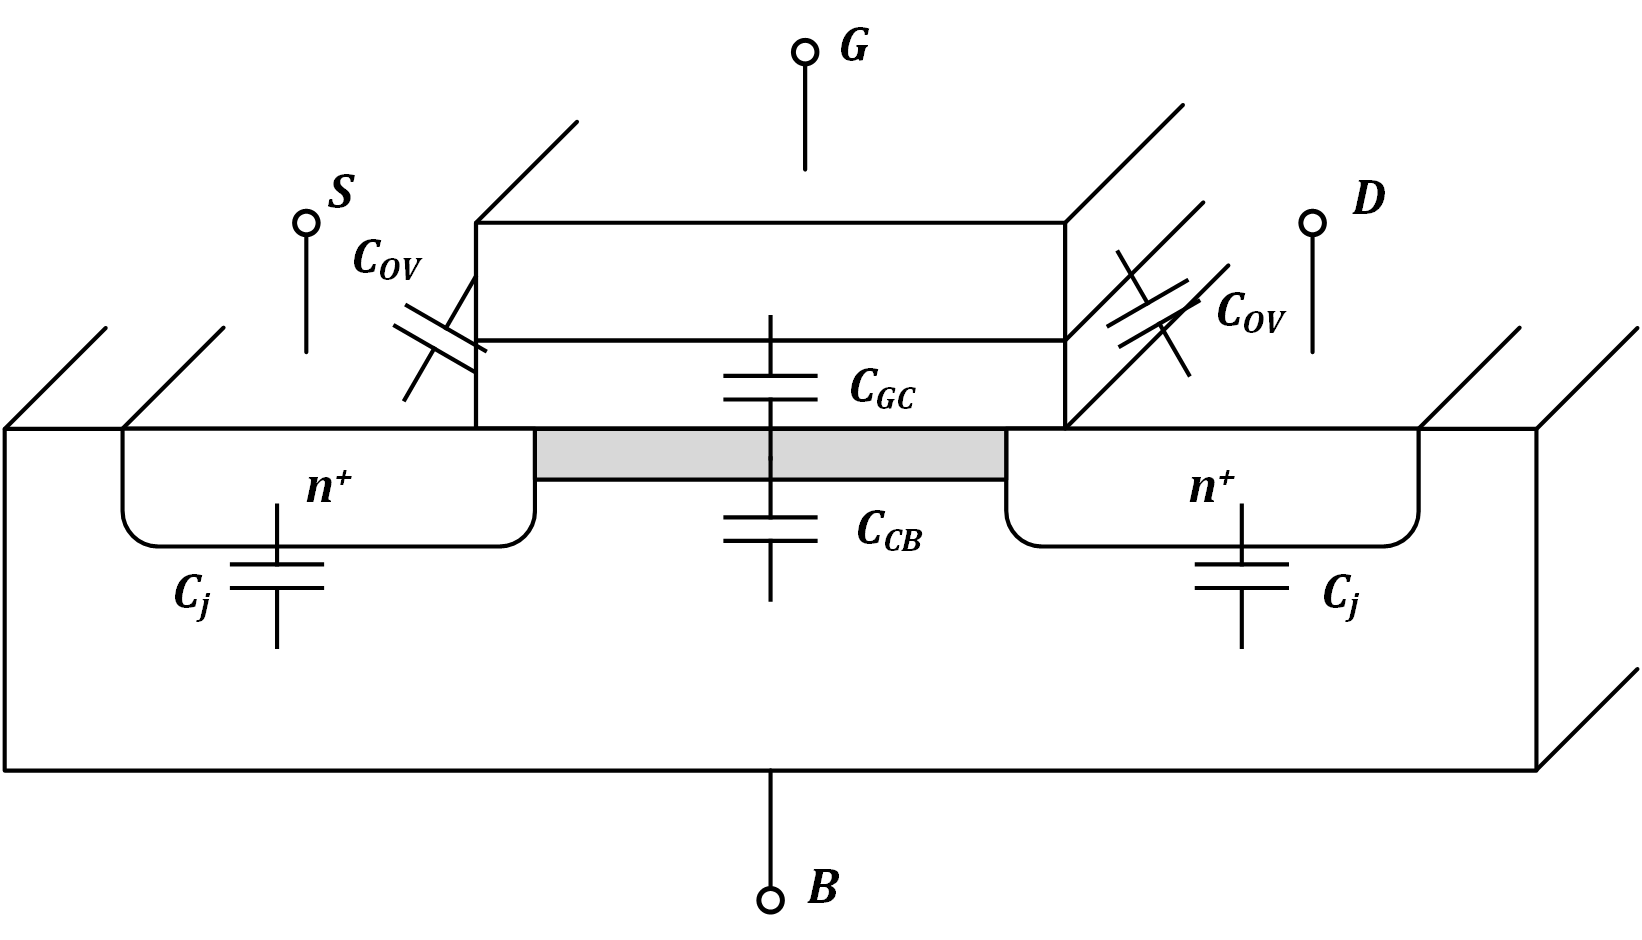
\includegraphics{MOS_capacitance.png}
\caption{MOS\_capacitance.png}
\end{figure}

    \begin{itemize}
\tightlist
\item
  MOS model comprises both intrinsic and extrinsic capacitances
\item
  Intrinsic capacitances (\(C_{GC}\), \(C_{GB}\)) are fundamental to
  device operation
\item
  Extrinsic capacitances (\(C_j\), \(C_{OV}\)) are incidental to its
  structure
\end{itemize}

    \hypertarget{intrinsic-capacitance-subthreshold}{%
\subsection{Intrinsic capacitance:
subthreshold}\label{intrinsic-capacitance-subthreshold}}

    \begin{figure}
\centering
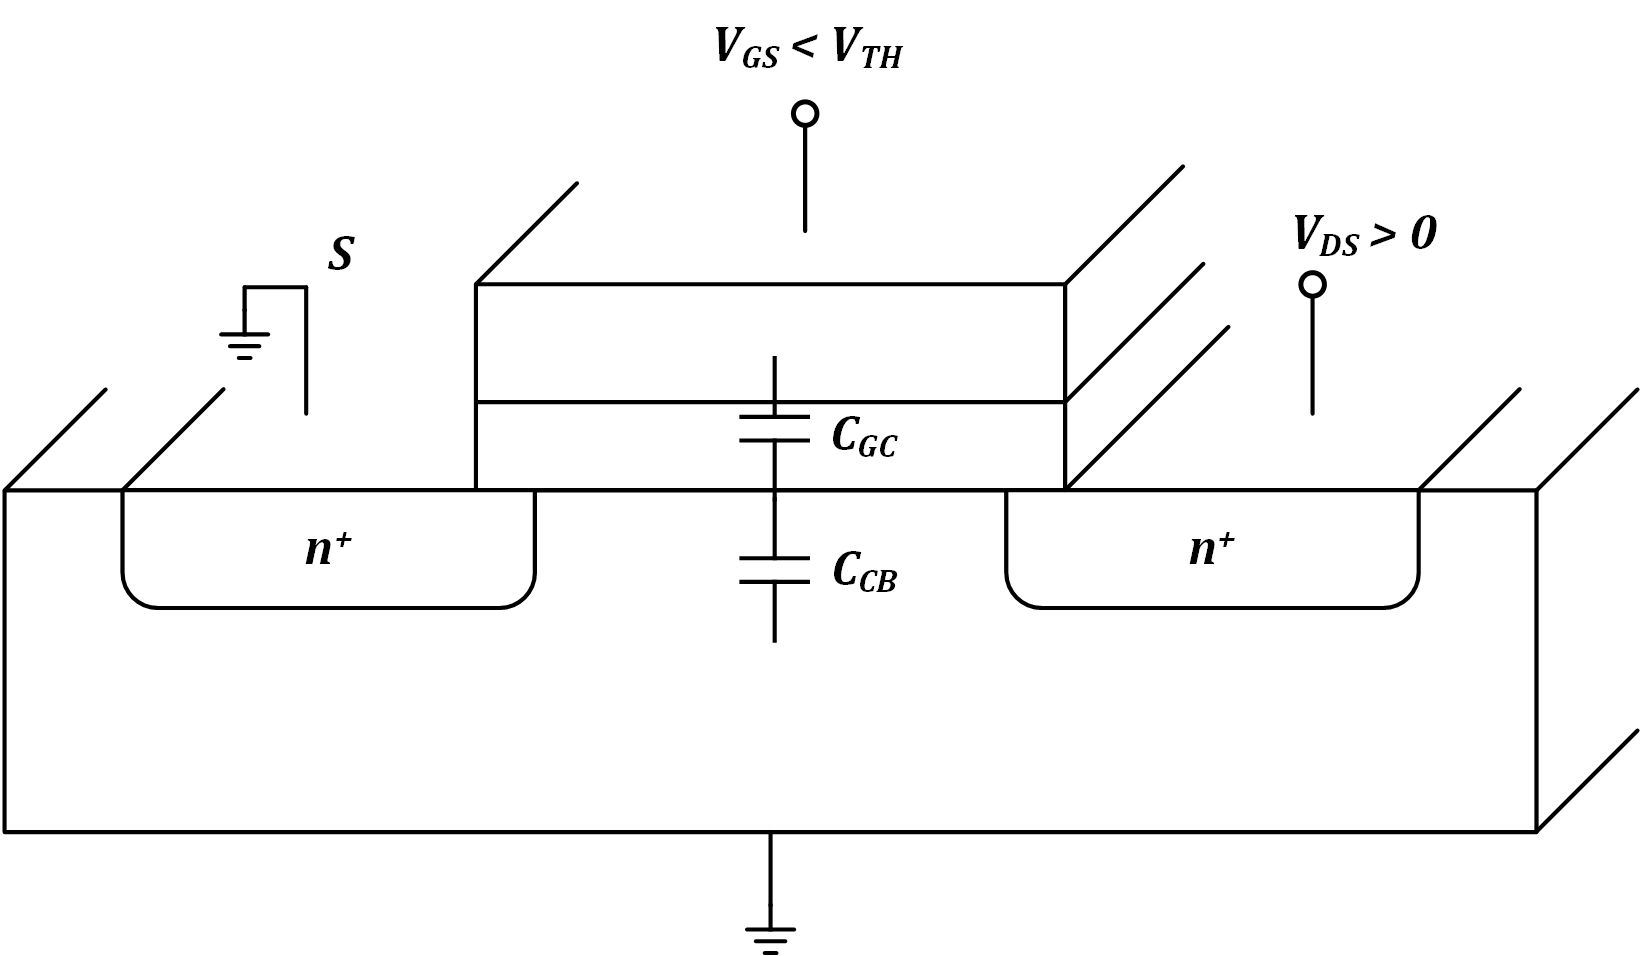
\includegraphics{subthreshold_capacitance.png}
\caption{subthreshold\_capacitance.png}
\end{figure}

    \begin{equation}
C_{CB} = WL \sqrt{\dfrac{q\epsilon_{Si}N_{sub}}{4 \phi_F}}
\end{equation}

\begin{equation}
C_{GC} = WLC_{ox}
\end{equation}

\begin{equation}
\boxed{C_G = \dfrac{C_{CB}C_{GC}}{C_{CB}+C_{GC}}}
\end{equation}

    \begin{itemize}
\tightlist
\item
  For \(V_{GS} < V_{th}\) no conductive channel exists between source
  and drain
\item
  \(C_{GC}\) and \(C_{CB}\) form a series capacitance
\item
  The ratio of \(C_{GC}\) to \(C_{CB}\) sets the factor \(n\) in the
  subthreshold drain current expression
\end{itemize}

    \hypertarget{intrinsic-capacitance-triode}{%
\subsection{Intrinsic capacitance:
triode}\label{intrinsic-capacitance-triode}}

    \begin{figure}
\centering
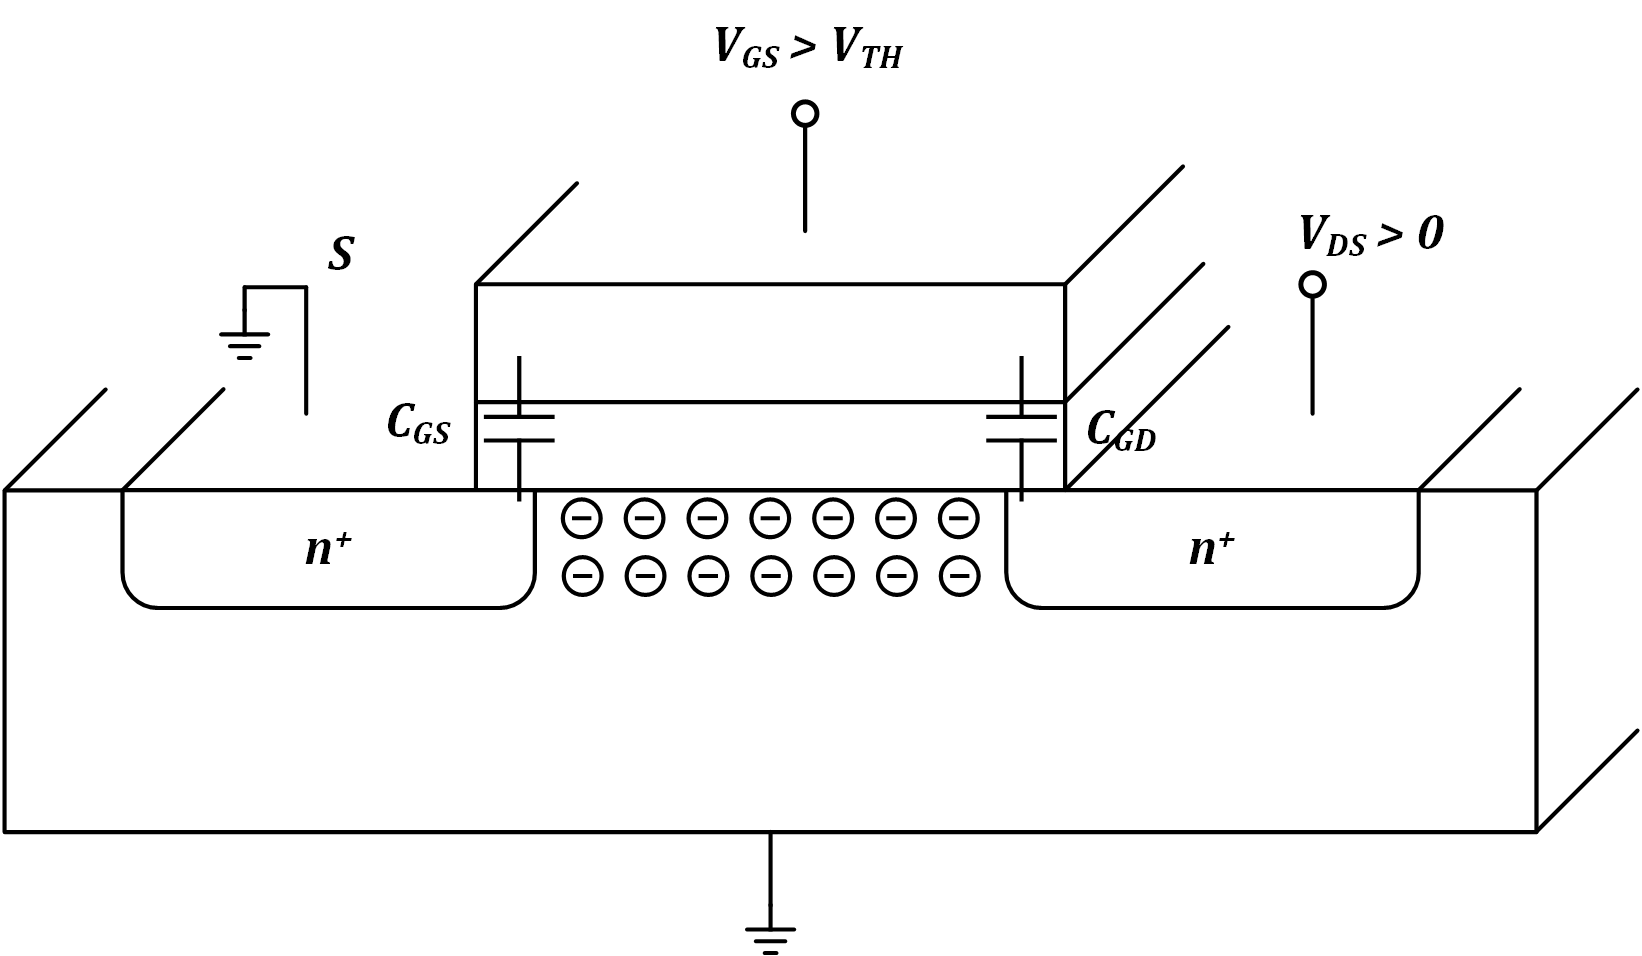
\includegraphics{triode_capacitance.png}
\caption{triode\_capacitance.png}
\end{figure}

    \begin{equation}
C_{GS} - C_{GD} = \dfrac{1}{2}WLC_{ox}
\end{equation}

\begin{equation}
\boxed{C_G = C_{GS} + C_{GD} = WLC_{ox}}
\end{equation}

    \begin{itemize}
\tightlist
\item
  In triode, the gate and channel form a parallel plate capacitance
  \(C{GC} = WL \epsilon_{ox}/t_{ox} = WLC_{ox}\)
\item
  Approximation using lumped capacitance \(C_{GS}\) and \(C_{GD}\)
  between gate-source and gate-drain terminals, each equal to
  \(C_{GC}/2\)
\item
  Depletion (junction) capacitance is typically negligible in comparison
\end{itemize}

    \hypertarget{intrinsic-capacitance-saturation}{%
\subsection{Intrinsic capacitance:
saturation}\label{intrinsic-capacitance-saturation}}

    \begin{figure}
\centering
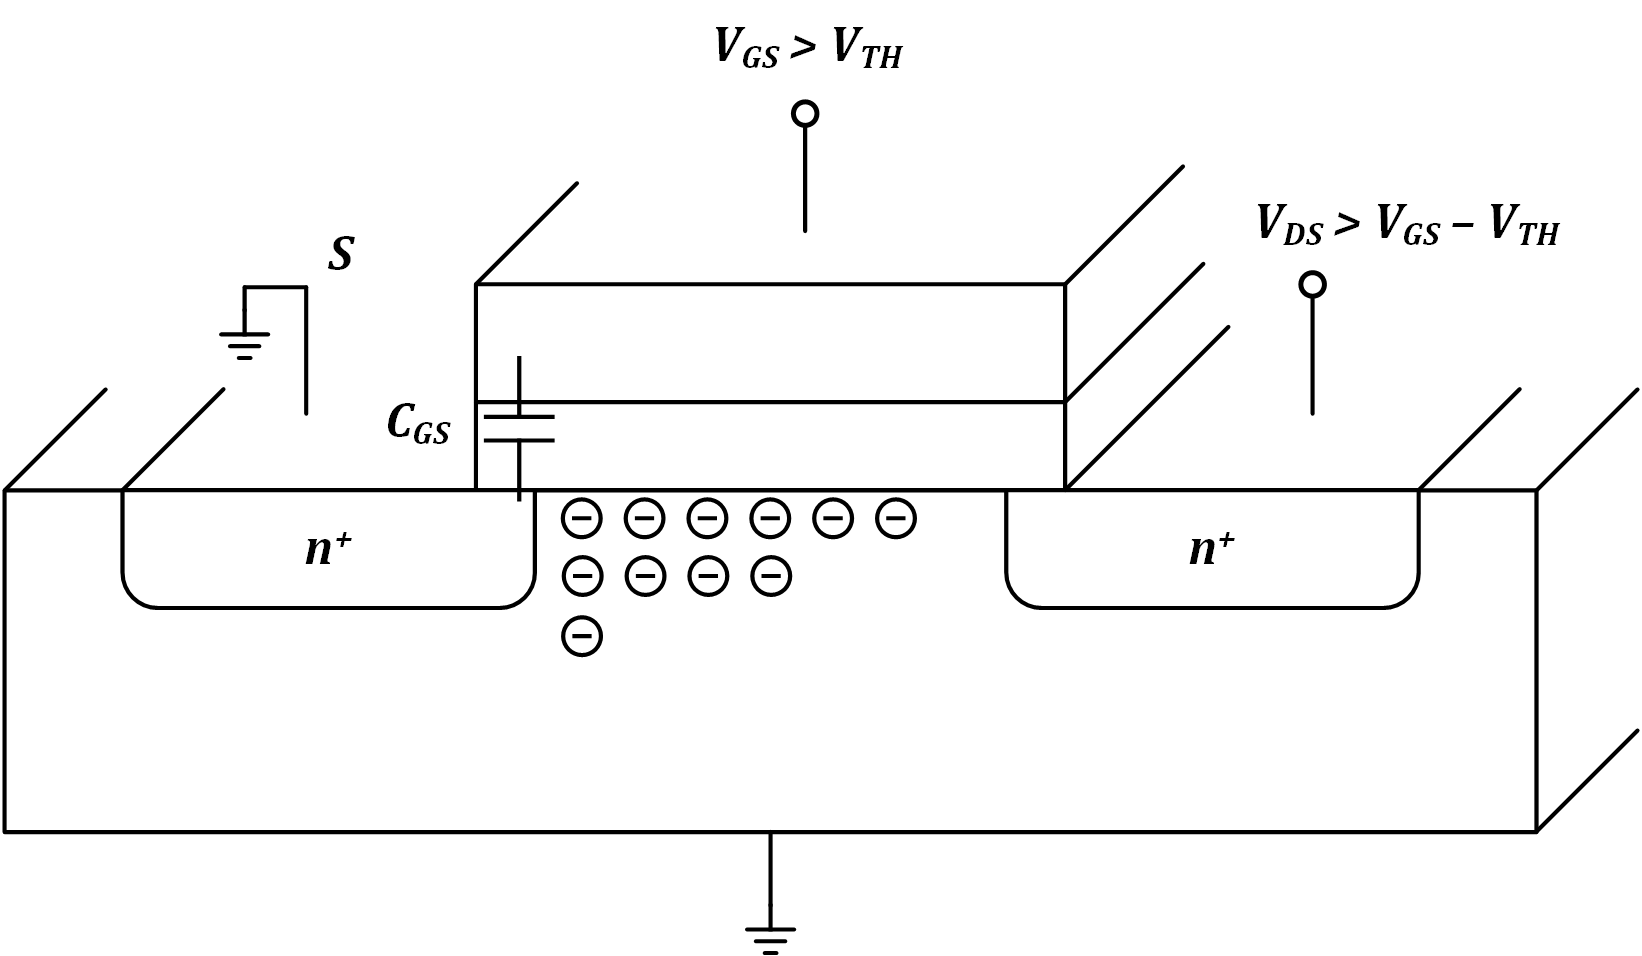
\includegraphics{saturation_capacitance.png}
\caption{saturation\_capacitance.png}
\end{figure}

    \begin{equation}
C_{GD} \approx 0
\end{equation}

\begin{equation}
\boxed{C_G = C_{GS} = \dfrac{2}{3}WLC_{ox}}
\end{equation}

    \begin{itemize}
\tightlist
\item
  In saturation, the ``bottom plate'' associated with \(C_{GC}\) isn't
  uniform along the channel
\item
  Detailed analysis gives \(C_{G} = C_{GS} = (2/3) WLC_{ox}\)
\item
  Drain voltage no longer affects channel charge, so \(C_{GD} = 0\)
\end{itemize}

    \hypertarget{extrinsic-capacitance-cov}{%
\subsection{Extrinsic capacitance
(COV)}\label{extrinsic-capacitance-cov}}

    \begin{figure}
\centering
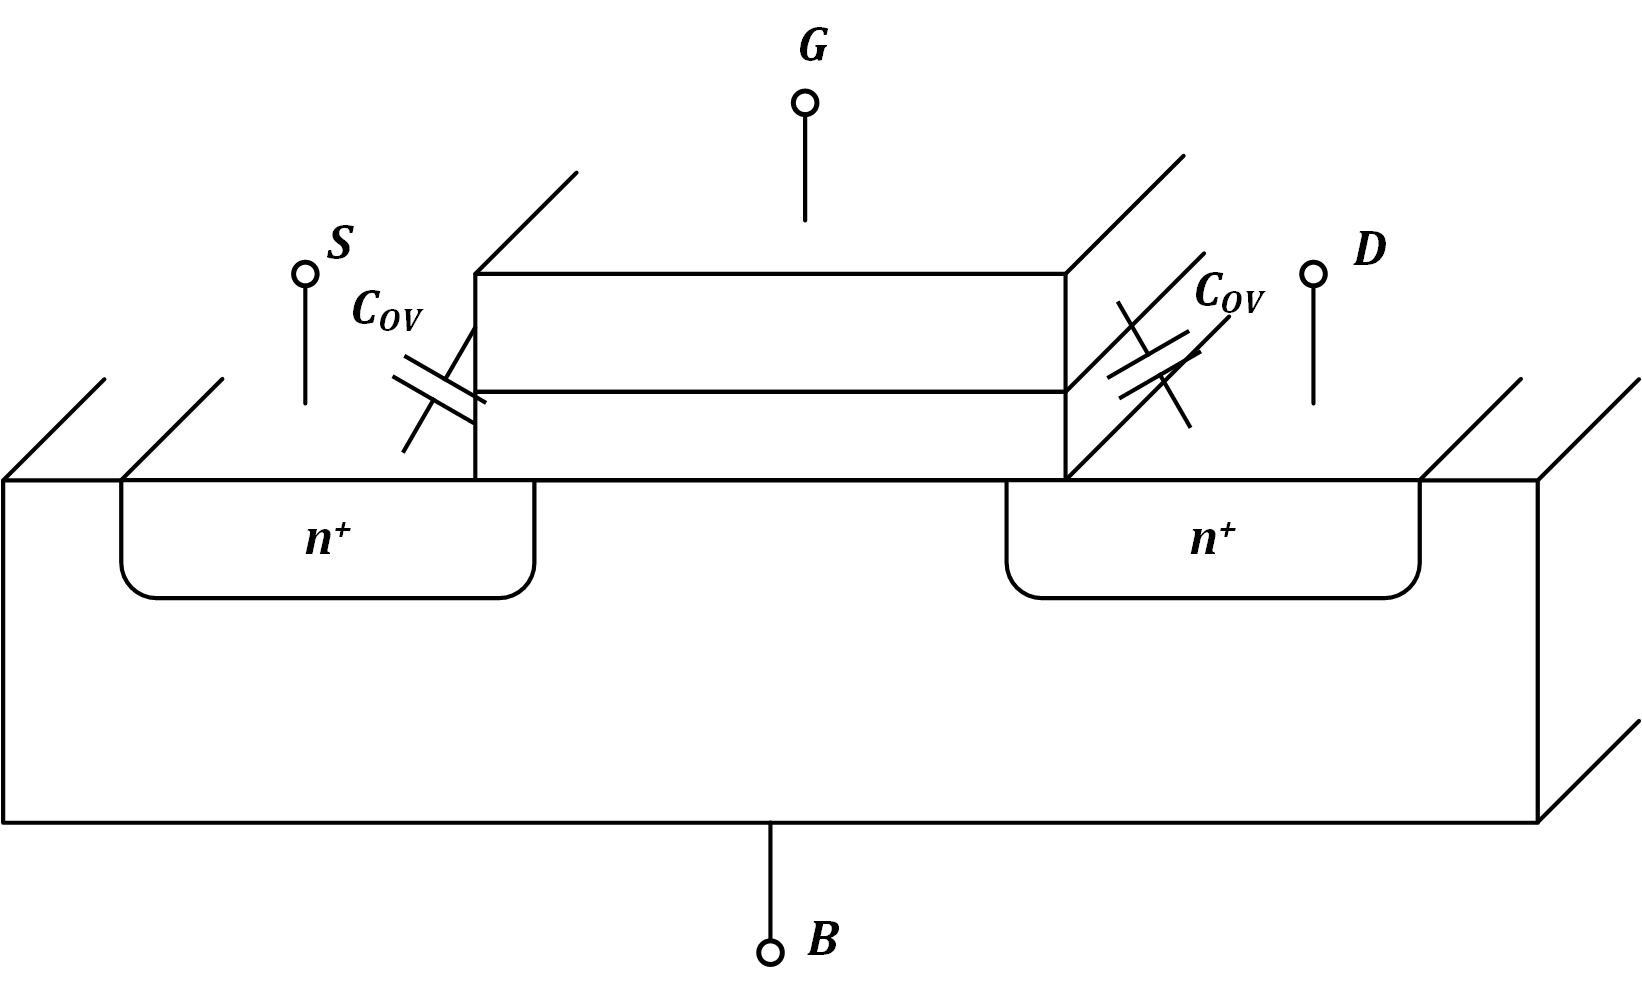
\includegraphics{overlap_capacitance.png}
\caption{overlap\_capacitance.png}
\end{figure}

    \begin{equation}
\boxed{C_{OV} = WC_{GD0}}
\end{equation}

\begin{equation}
[C_{GD0}] = F/m
\end{equation}

    \begin{itemize}
\tightlist
\item
  Due to diffusion during device fabrication, both source and drain
  regions extend under the gate by \(\Delta L\)
\item
  The overlap between gate polysilicon and S/D regions results in a
  capacitance-per-unit-width \(C_{OV}\)
\item
  ``Fringe'' electric fields also contribute to the capacitance
\end{itemize}

    \hypertarget{extrinsic-capacitance-cj}{%
\subsection{Extrinsic capacitance (Cj)}\label{extrinsic-capacitance-cj}}

    \begin{figure}
\centering
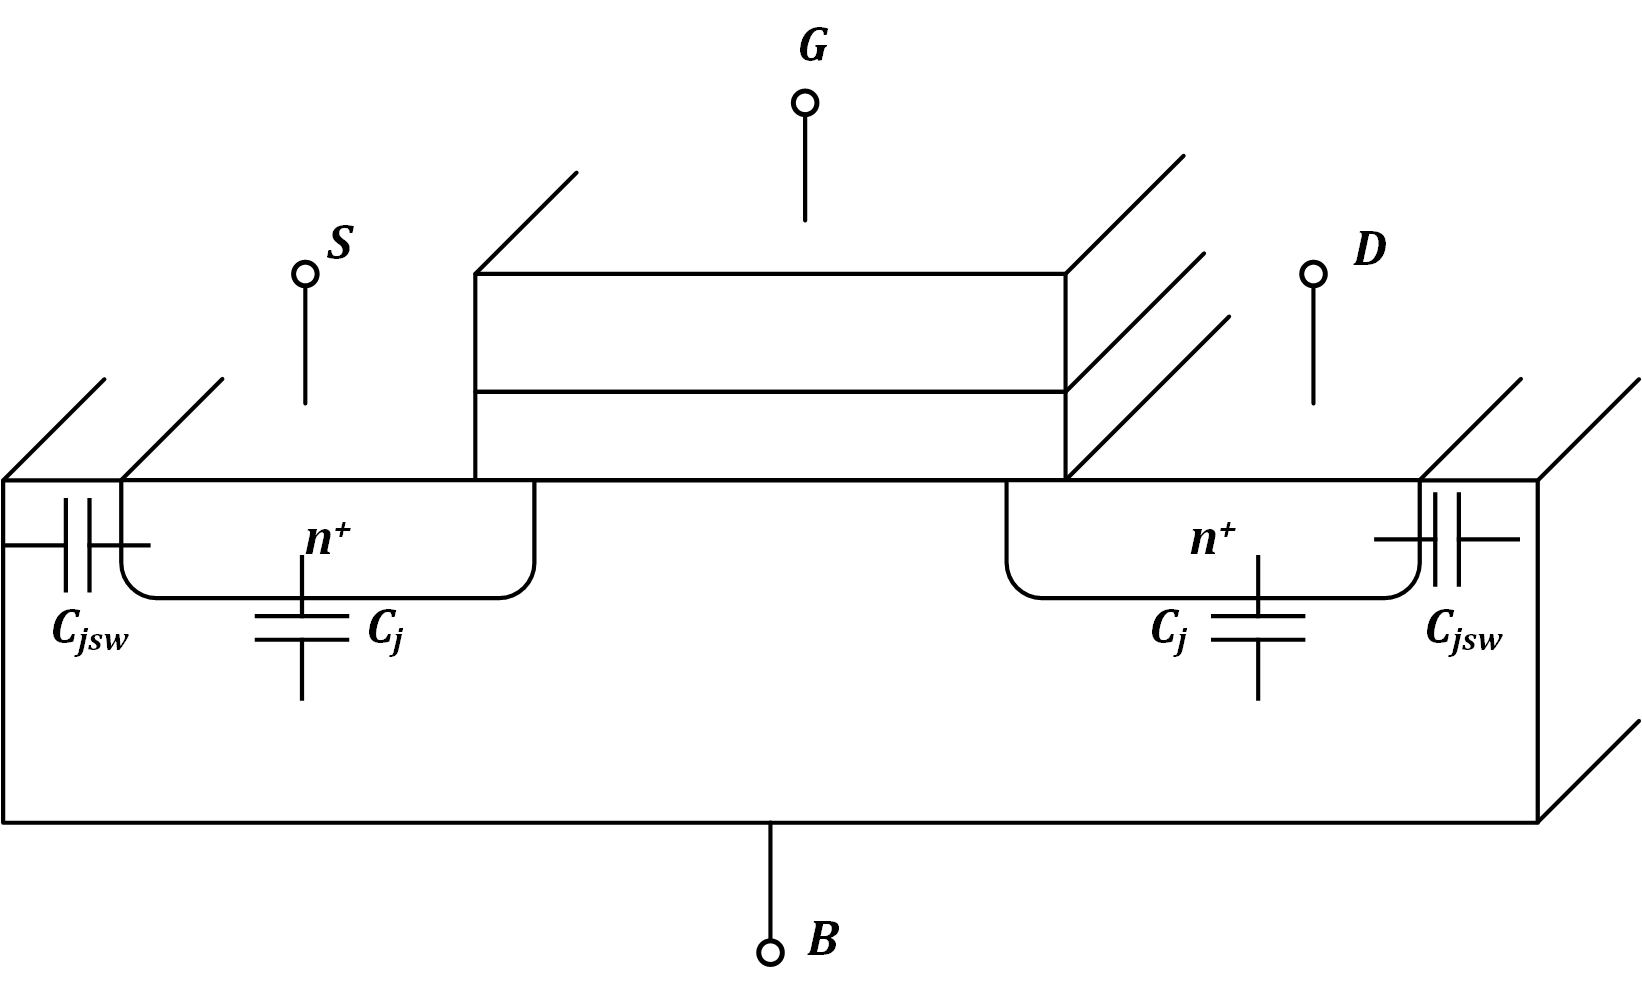
\includegraphics{junction_capacitance.png}
\caption{junction\_capacitance.png}
\end{figure}

    \begin{equation}
\boxed{C_{j,tot} = A_{SD}C_j + P_{SD}C_{jsw}}
\end{equation}

\begin{equation}
[C_j] = F/m^2
\end{equation}

\begin{equation}
[C_{jsw}] = F/m
\end{equation}

    \begin{itemize}
\tightlist
\item
  Source and drain regions form \(pn\)-junction capacitances with the
  bulk semiconductor (\(C_{SB}\), \(C_{DB}\))
\item
  These junctions are nominally reverse-biased (for an NMOS transistor,
  the bulk is biased at the most negative potential in the system,
  typically ground)
\item
  Similarly for PMOS devices, the \(n\)-type bulk is biased at
  \(V_{DD}\), reverse-biasing the junction
\item
  Junction capacitances scale with transistor width
\end{itemize}

    \hypertarget{mos-saturation-model}{%
\subsection{MOS saturation model}\label{mos-saturation-model}}

    \begin{figure}
\centering
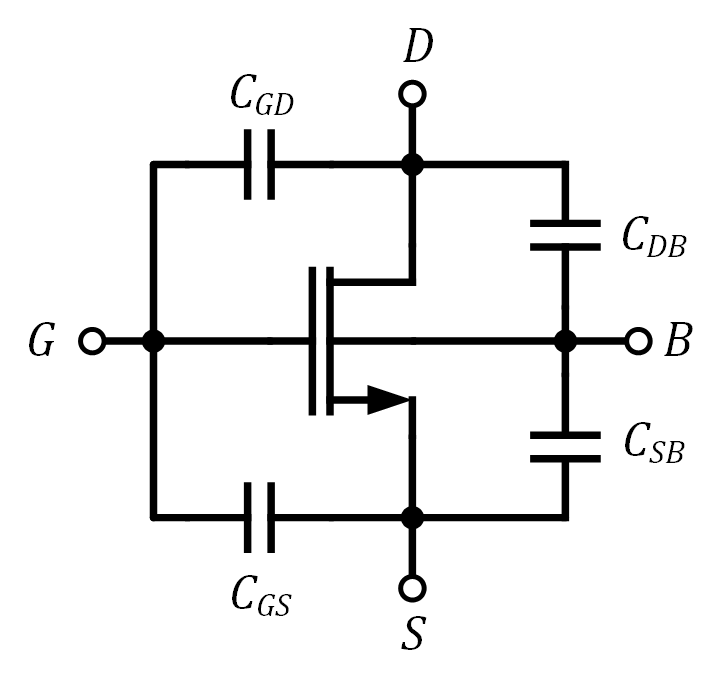
\includegraphics{MOS_cap_saturation.png}
\caption{MOS\_cap\_saturation.png}
\end{figure}

    \begin{itemize}
\tightlist
\item
  MOS capacitance in saturation is largely dominated by \(C_{GS}\), so
  in many cases other capacitances are neglected in hand calculations
\item
  All intrinsic/extrinsic capacitances increase with gate dimensions,
  such that larger transistors exhibit higher capacitance
\item
  The ultimate limit of usability of the MOS transistor as a gain
  element is determined by intrinsic device capacitance, and is
  described by the transit frequency (\(f_t\)) of a device
\end{itemize}

    \hypertarget{small-signal-mos-model-ac}{%
\subsection{Small-signal MOS model
(AC)}\label{small-signal-mos-model-ac}}

    \begin{figure}
\centering
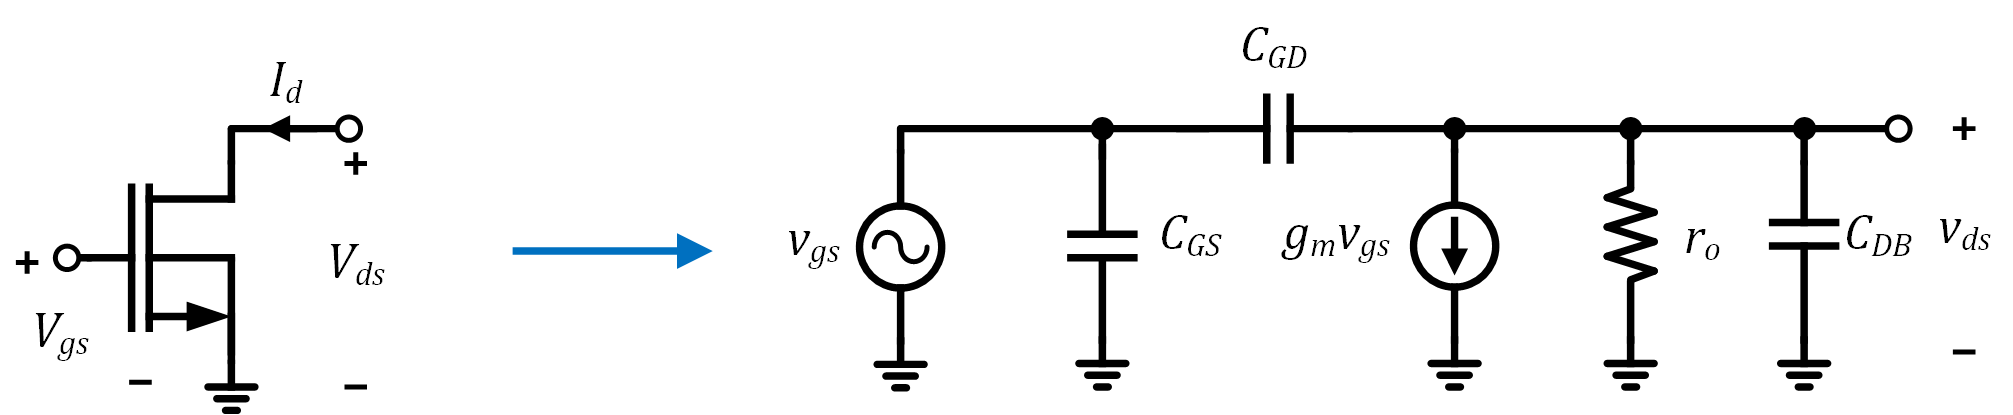
\includegraphics{AC_small_signal.png}
\caption{AC\_small\_signal.png}
\end{figure}

    \begin{itemize}
\tightlist
\item
  In analog design, we typically use MOS devices in a common-source or
  current-source configuration
\item
  Small-signal models quickly become unwieldy due to the large number of
  devices/parameters
\item
  Again, we should use the simplest model that is accurate enough for
  our purposes!
\end{itemize}

    \hypertarget{common-source-amplifier}{%
\subsection{Common-source amplifier}\label{common-source-amplifier}}

    \begin{figure}
\centering
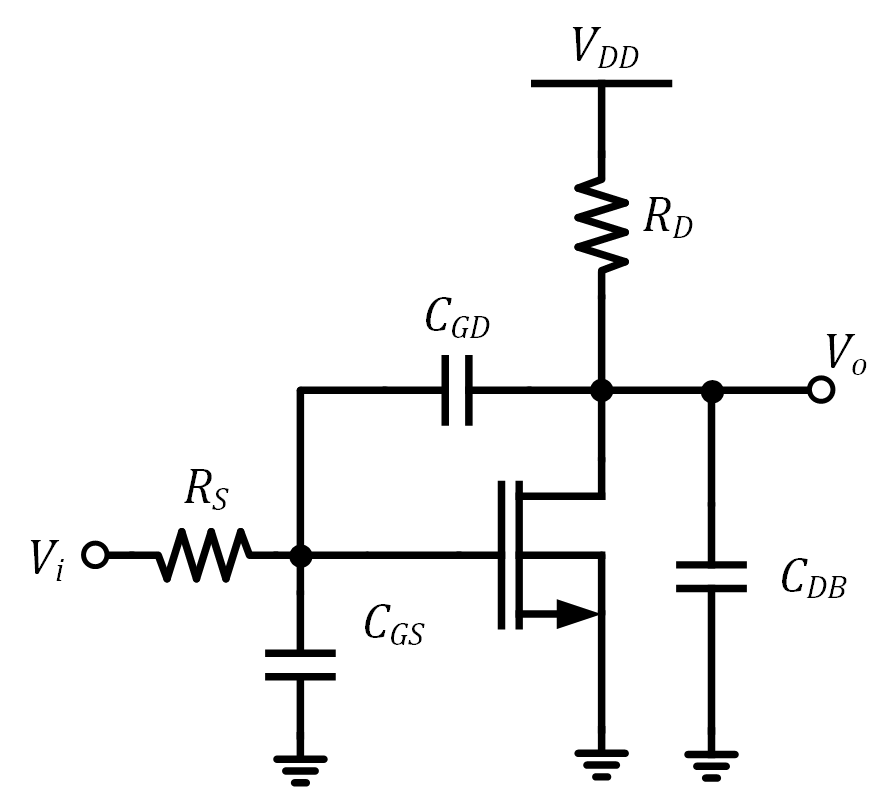
\includegraphics{common_source_AC.png}
\caption{common\_source\_AC.png}
\end{figure}

    \begin{itemize}
\tightlist
\item
  We are interested in finding \(v_o/v_i\) (small-signal gain) as a
  function of frequency:
\end{itemize}

\begin{equation}
A_v(s) =\dfrac{v_o}{v_i}(s) = ?
\end{equation} - Device capacitance plays a role, as do other
capacitances (e.g.~load capacitors or subsequent stage parasitics) - For
now, we'll perform our analysis with only the MOS capacitances

    \hypertarget{common-source-small-signal-model}{%
\subsection{Common-source small-signal
model}\label{common-source-small-signal-model}}

    \begin{figure}
\centering
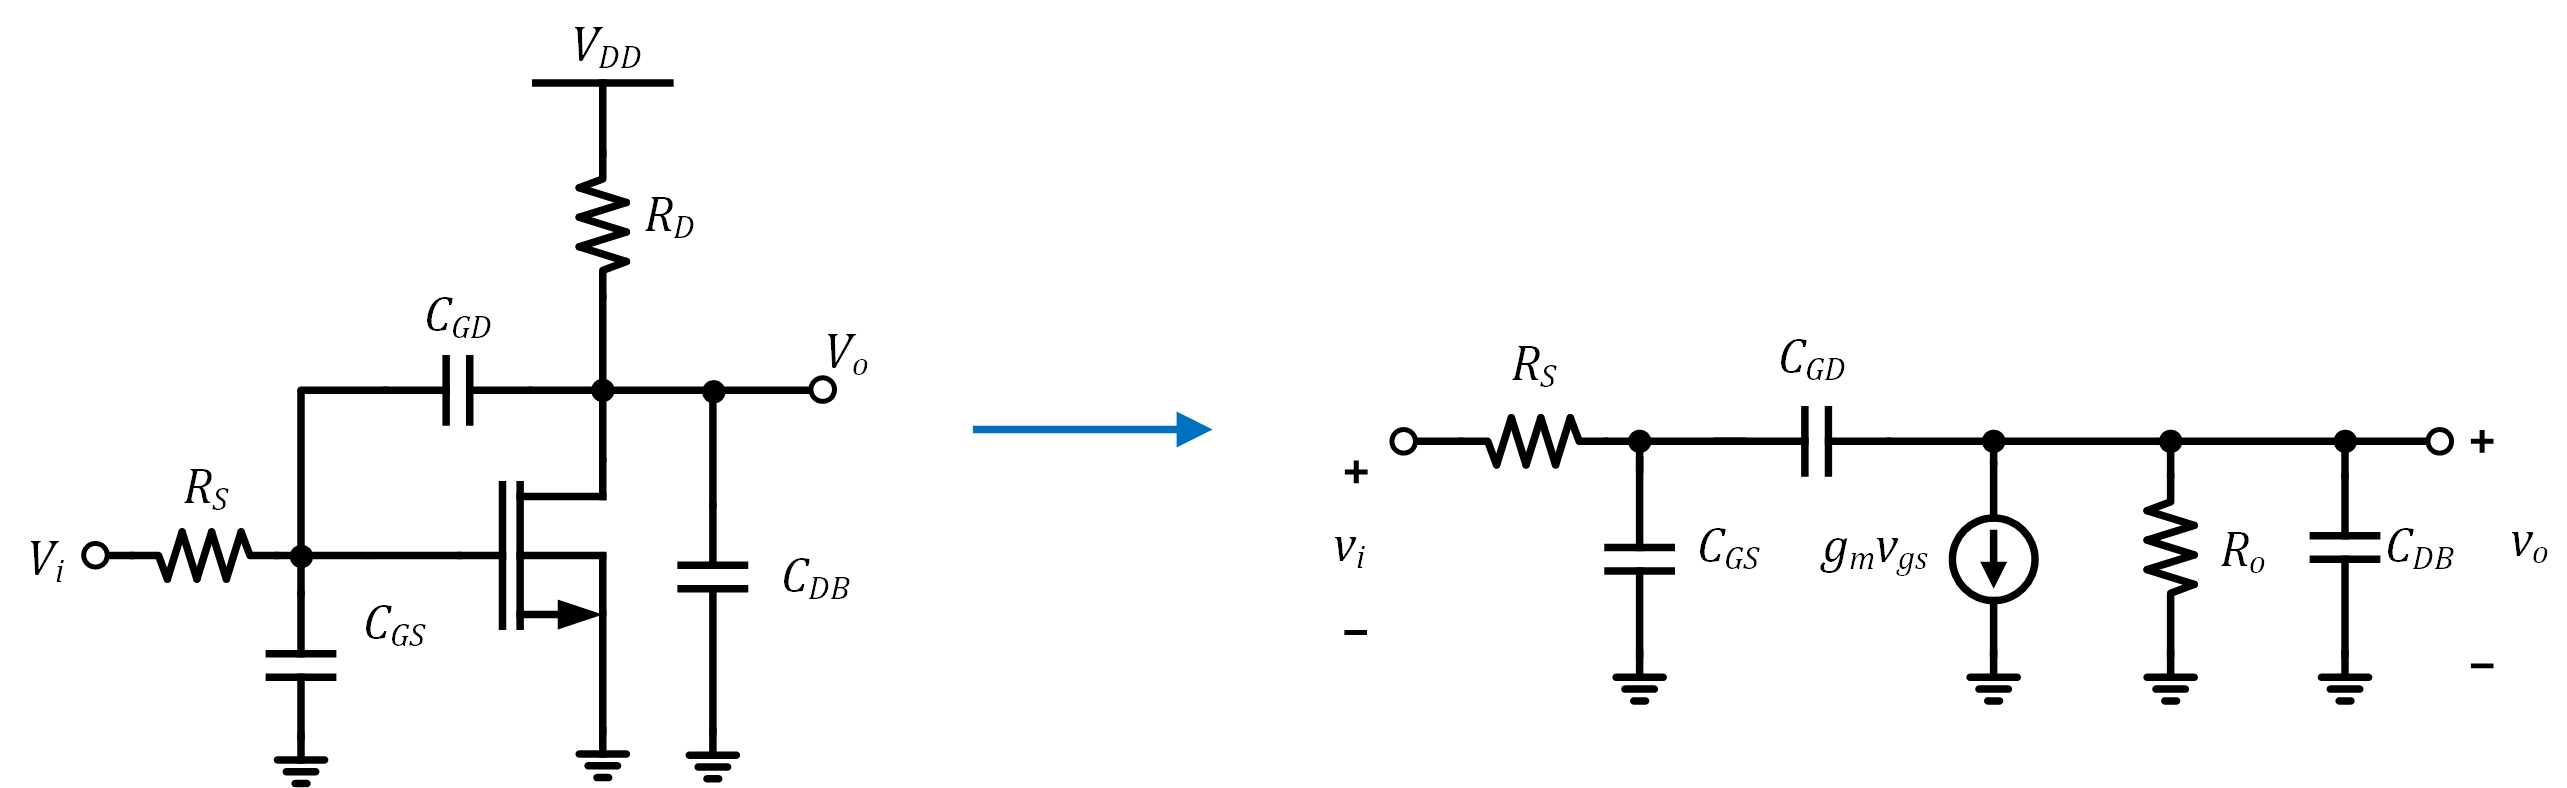
\includegraphics{common_source_small_signal_model.png}
\caption{common\_source\_small\_signal\_model.png}
\end{figure}

    \begin{itemize}
\tightlist
\item
  Complete small-signal model includes \(g_m\), \(r_o\), and MOS
  capacitances
\item
  Small-signal analysis is a bit more involved that at DC, but hand
  analysis is still manageable for one or two devices
\item
  The output resistance is given by \(R_o = r_o||R_D\)
\item
  \(R_S\) represents the output (Thevenin) resistance of the previous
  stage
\end{itemize}

    \hypertarget{complete-small-signal-analysis}{%
\subsection{Complete small-signal
analysis}\label{complete-small-signal-analysis}}

    \begin{figure}
\centering
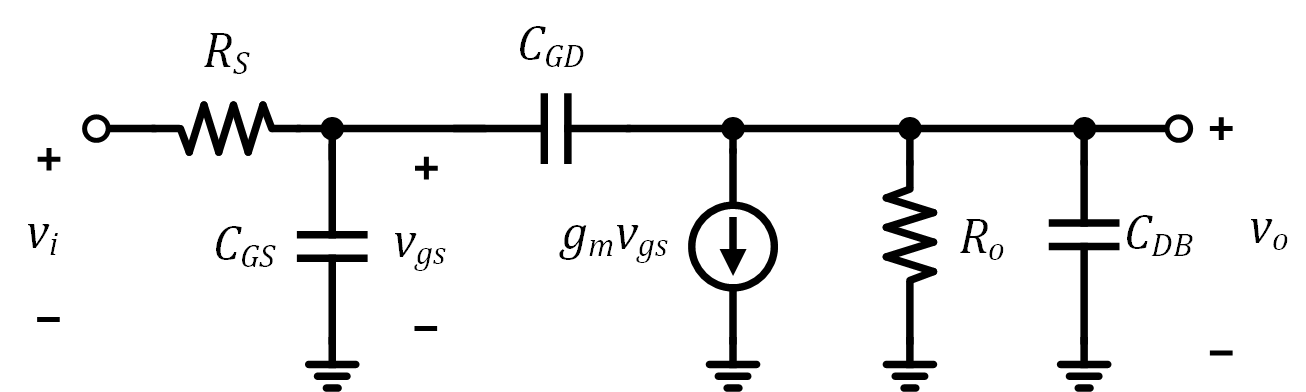
\includegraphics{common_source_small_signal.png}
\caption{common\_source\_small\_signal.png}
\end{figure}

    \begin{equation}
\dfrac{v_i - v_{gs}}{R_S} = sC_{GS}v_{gs} + sC_{GD}(v_{gs} - v_o)
\end{equation}

\begin{equation}
sC_{GD}(v_{gs} - v_o) = g_m v_{gs} + v_o\left(sC_{GB} + \dfrac{1}{R_o}\right)
\end{equation}

    \begin{itemize}
\tightlist
\item
  This system of equations is deceptively simple!
\item
  Let's solve for \(v_o/v_i\)\ldots{}
\end{itemize}

    \begin{itemize}
\tightlist
\item
  The small-signal AC model is used to obtain two KCL equations, one for
  the gate node and one for the drain
\end{itemize}

\begin{equation}
\dfrac{v_i - v_{gs}}{R_S} = sC_{GS}v_{gs} + sC_{GD}(v_{gs} - v_o)
\end{equation}

\begin{equation}
sC_{GD}(v_{gs} - v_o) = g_m v_{gs} + v_o\left(sC_{GB} + \dfrac{1}{R_o}\right)
\end{equation}

\begin{itemize}
\tightlist
\item
  From this pair of equations we obtain
\end{itemize}

\begin{equation}
A_v(s) =\dfrac{v_o}{v_i} = \dfrac{(sC_{GD} - g_m)R_o}{R_S R_o\xi s^2 + [R_S(1+g_mR_o)C_{GD} + R_SC_{GS}+R_D(C_{GD} + C_{DB})]s+1}
\end{equation}

\begin{itemize}
\tightlist
\item
  where the term \(\xi\) is given by
\end{itemize}

\begin{equation}
\xi = C_{GS}C_{GD} + C_{GS}C_{DB} + C_{GD}C_{DB}
\end{equation}

    \hypertarget{low-frequency-response}{%
\subsection{Low-frequency response}\label{low-frequency-response}}

    \begin{figure}
\centering
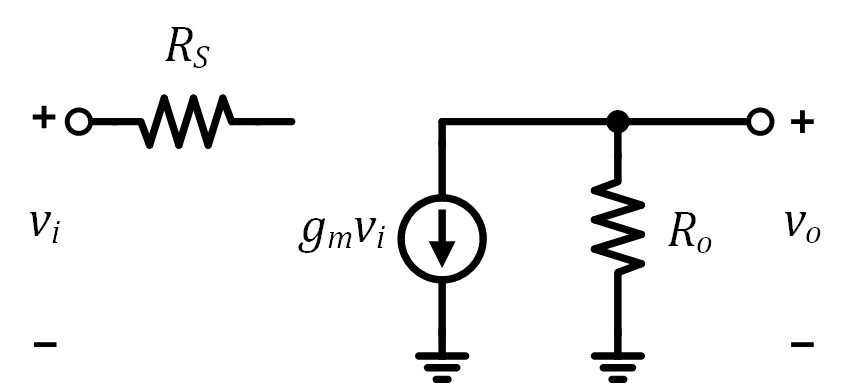
\includegraphics{common_source_LF.png}
\caption{common\_source\_LF.png}
\end{figure}

    \begin{itemize}
\tightlist
\item
  To understand the performance of the amplifier at low frequencies, we
  can ``open-circuit'' capacitances in the small-signal model
\item
  The transfer function of the common-source amplifier is given by
\end{itemize}

\begin{equation}
A_v(s) = \dfrac{(sC_{GD} - g_m)R_o}{R_S R_o\xi s^2 + [R_S(1+g_mR_o)C_{GD} + R_SC_{GS}+R_o(C_{GD} + C_{DB})]s+1}
\end{equation}

\begin{itemize}
\tightlist
\item
  If we let \(s\rightarrow0\), we obtain the low-frequency (DC) response
\end{itemize}

\begin{equation}
\lim_{s\rightarrow 0}{A_v(s)} = -g_m R_o = -g_m r_o || R_D \approx \boxed{-g_m R_D}
\end{equation}

    \hypertarget{high-frequency-response}{%
\subsection{High-frequency response}\label{high-frequency-response}}

    \begin{figure}
\centering
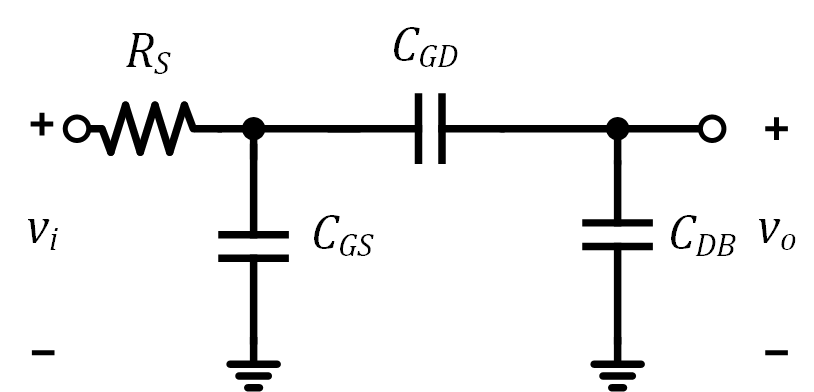
\includegraphics{common_source_HF.png}
\caption{common\_source\_HF.png}
\end{figure}

    \begin{itemize}
\tightlist
\item
  To assess the behavior of the circuit at high frequencies, we note
  that capacitances will shunt (i.e.~short-circuit) other circuit
  elements due to the fact that their impedances are decreasing with
  frequency
\item
  As \(s \rightarrow \infty\) in the transfer function, we obtain
\end{itemize}

\begin{equation}
\lim_{s\rightarrow \infty}{A_v(s)} = \dfrac{C_{GD}}{sR_S(C_{GS}C_{GD} + C_{GS}C_{DB} + C_{GD}C_{DB})}
\end{equation}

    \hypertarget{common-source-dominant-pole}{%
\subsection{Common-source dominant
pole}\label{common-source-dominant-pole}}

    \begin{itemize}
\tightlist
\item
  The common-source transfer function can be expressed as
\end{itemize}

\begin{align}
A_v(s) &= \dfrac{(sC_{GD} - g_m)R_o}{R_S R_o\xi s^2 + [R_S(1+g_mR_o)C_{GD} + R_SC_{GS}+R_o(C_{GD} + C_{DB})]s+1} \\
\\
&=\dfrac{(sC_{GD} - g_m)R_o}{\dfrac{s^2}{\omega_{p1}\omega_{p2}} + \left(\dfrac{1}{\omega_{p1}}+\dfrac{1}{\omega_{p2}} \right)s + 1
}\end{align}

\begin{itemize}
\tightlist
\item
  If we assume that \(\omega_{p1} << \omega_{p2}\) (the so-called
  ``dominant-pole approximation''), \(\omega_{p1}\) can be approximated
  as
\end{itemize}

\begin{equation}
\omega_{p1} \approx \dfrac{1}{R_S(1+g_mR_o)C_{GD} + R_SC_{GS}+R_D(C_{GD} + C_{DB})}
\end{equation}

    \hypertarget{common-source-frequency-response}{%
\subsection{Common-source frequency
response}\label{common-source-frequency-response}}

    \begin{itemize}
\tightlist
\item
  By making some assumptions (i.e.~the dominant pole approximation) we
  were able to arrive at some results that provide some design insight
\item
  However, this was only possible after somewhat lengthy (small-signal)
  analysis, and this even for a circuit with only a single transistor
\item
  Let's look at a couple of useful methods for simplifying the frequency
  response analysis of MOS circuits: Miller's Theorem and Zero-Value
  Time Constant Analysis
\end{itemize}

    \hypertarget{millers-theorem}{%
\subsection{Miller's Theorem}\label{millers-theorem}}

    \begin{figure}
\centering
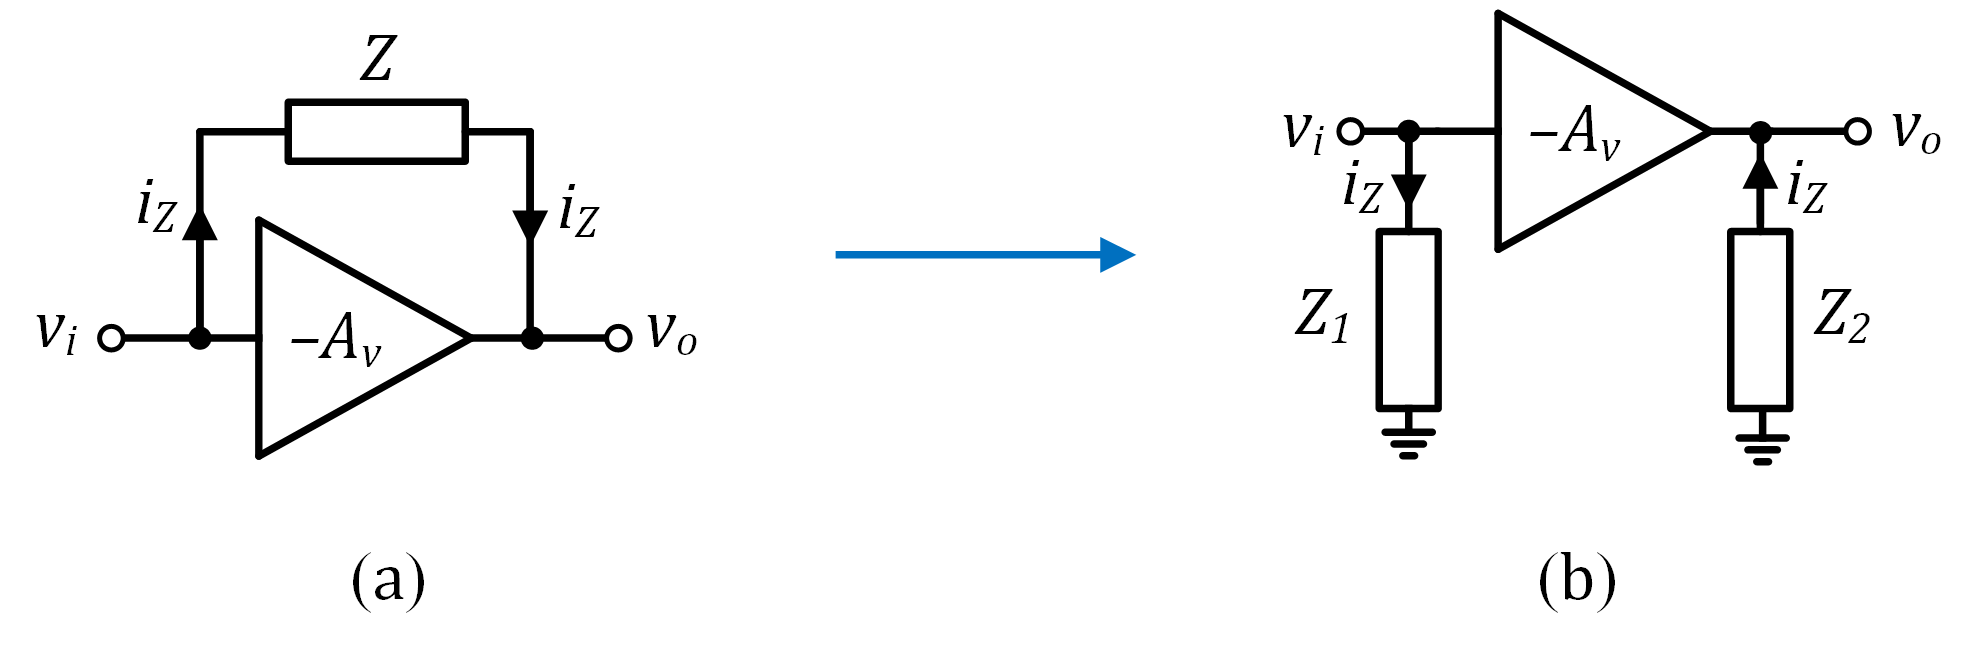
\includegraphics{Miller_theorem.png}
\caption{Miller\_theorem.png}
\end{figure}

    \begin{itemize}
\tightlist
\item
  Theorem: If Circuit (a) can be represented as Circuit (b), then
  \(Z_1\) and \(Z_2\) can be given by
\end{itemize}

\begin{equation}
Z_1 = \dfrac{Z}{1+A_v} \:\:\:\:\:\:\:\:\:\:\:\: Z_2 = Z\cdot (1+A_v)
\end{equation}

    \begin{figure}
\centering
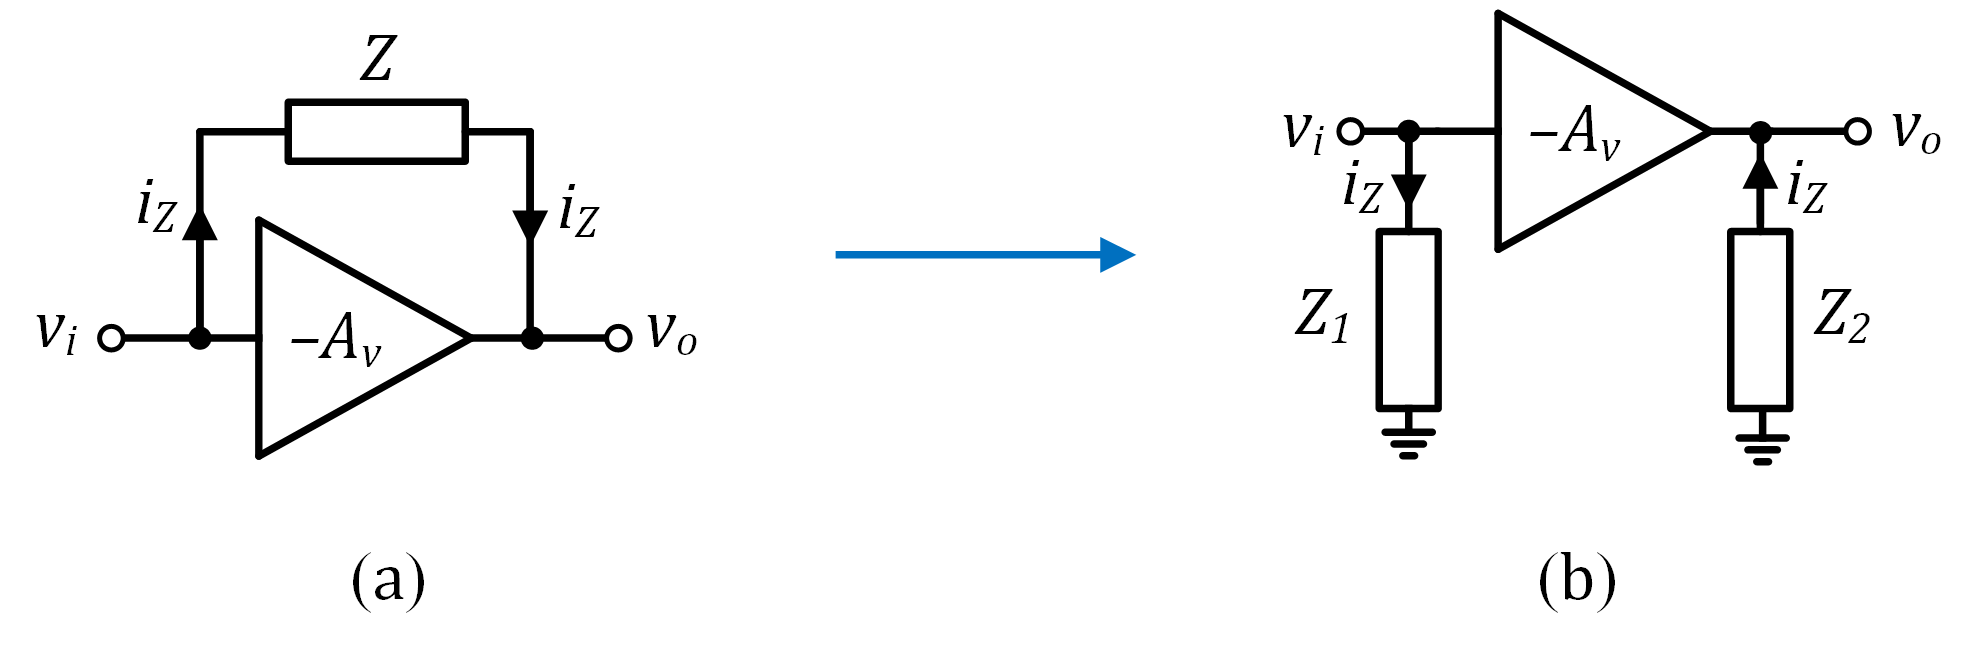
\includegraphics{Miller_theorem.png}
\caption{Miller\_theorem.png}
\end{figure}

    \begin{itemize}
\tightlist
\item
  The current through \(Z\), \(i_Z\), is given by
\end{itemize}

\begin{equation}
i_Z = \dfrac{v_i - v_o}{Z} = \dfrac{v_i(1 + A_v)}{Z} = \dfrac{-v_o \left(\dfrac{1}{A_v}+1\right)}{Z}
\end{equation}

\begin{itemize}
\tightlist
\item
  We can then relate \(Z_1\) and \(Z_2\) to \(i_Z\) and the node
  voltages \(v_i\) and \(v_o\)
\end{itemize}

\begin{equation}
Z_1 = \dfrac{v_i}{i_Z} = \dfrac{Z}{1+A_v} \:\:\:\:\:\:\:\:\:\:\:\: Z_2 = -\dfrac{v_o}{i_Z} = \dfrac{Z}{\dfrac{1}{A_v}+1} = \dfrac{A_v Z}{A_v + 1}
\end{equation}

    \begin{figure}
\centering
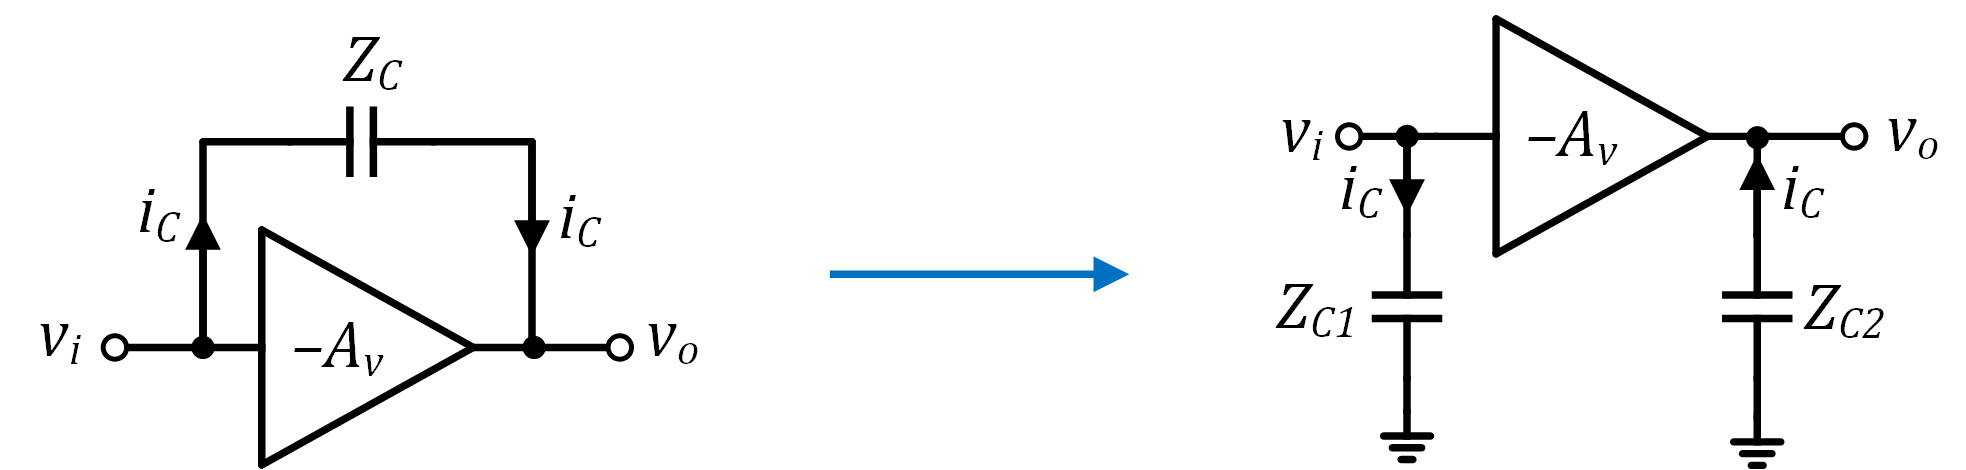
\includegraphics{miller_capacitance.png}
\caption{miller\_capacitance.png}
\end{figure}

    \begin{equation}
Z_{C1} = \dfrac{Z_C}{1+A_v} = \dfrac{1}{sC(1+A_v)} = \dfrac{1}{sC_1}
\end{equation}

\begin{equation}
\boxed{C_1 = (1+A_v) \cdot C \approx A_v \cdot C}
\end{equation}

    \begin{equation}
Z_{C2} = \dfrac{A_vZ_C}{1+A_v} = \dfrac{A_v}{sC(1+A_v)} = \dfrac{1}{sC_2}
\end{equation}

\begin{equation}
\boxed{C_2 = \dfrac{(1+A_v) \cdot C}{A_v} \approx C}
\end{equation}

    \begin{itemize}
\tightlist
\item
  Due to the amplification of \(v_i\) by \(A_v\), the voltage across
  capacitor \(C\) is increased by a factor \(A_v\)
\item
  This increases the current through \(C\) by the same factor (\(A_v\)),
  increasing the \emph{effective} capacitance ``seen'' by \(v_i\)
  (\(C_1\)) by \(A_v\)
\item
  From the perspective of \(v_o\), \(v_i\) appears as a small-signal
  ground, so the effective capacitance for \(v_o\) (\(C_2\)) is just
  \(C\)
\end{itemize}

    \hypertarget{common-source-miller-approximation}{%
\subsection{Common-source Miller
approximation}\label{common-source-miller-approximation}}

    \begin{figure}
\centering
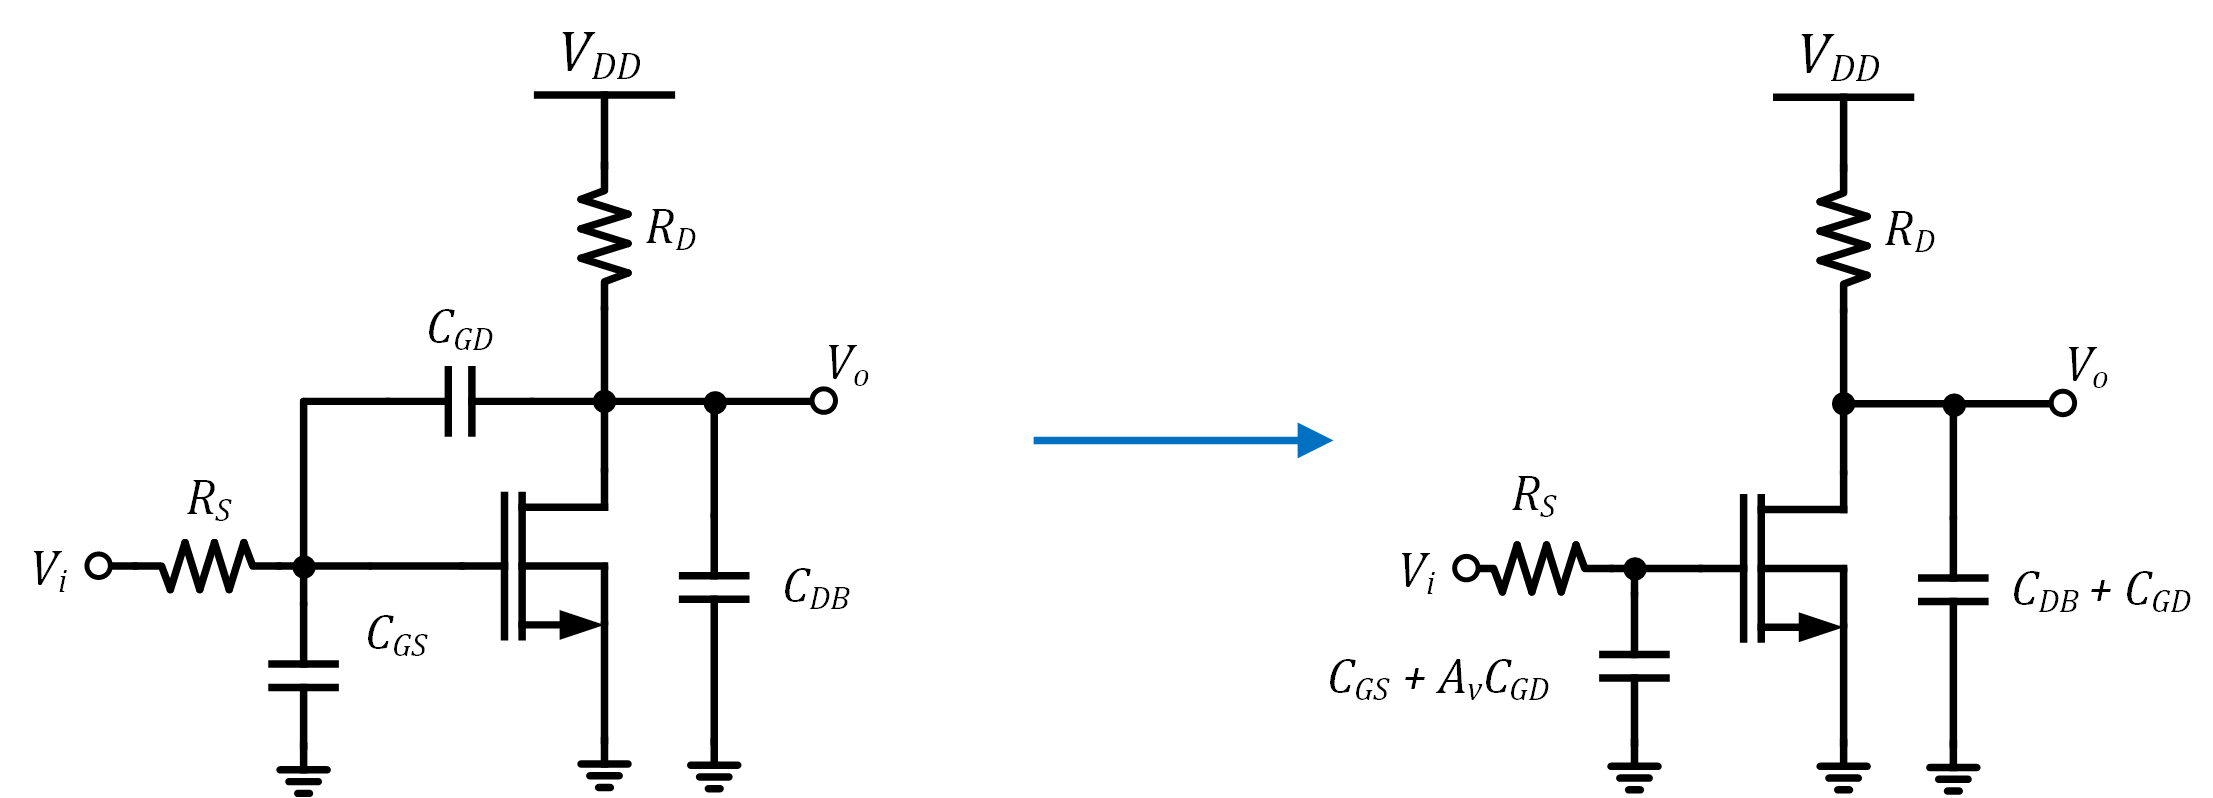
\includegraphics{common_source_miller_approximation.png}
\caption{common\_source\_miller\_approximation.png}
\end{figure}

    \begin{itemize}
\tightlist
\item
  By applying Miller's Theorem to the common-source amplifier, we
  greatly simplify the analysis of its frequency response
\item
  Note that in using Miller's approximation, we neglect a zero in the
  transfer function, as well as interaction between the input and output
  nodes of the amplifier
\end{itemize}

    \hypertarget{input-and-output-poles}{%
\subsection{Input and output poles}\label{input-and-output-poles}}

    \begin{itemize}
\tightlist
\item
  The input pole is given by
\end{itemize}

\begin{equation}
\omega_{p1} \approx \dfrac{1}{R_S( C_{GS} + A_v C_{GD}) }
\end{equation}

\begin{itemize}
\tightlist
\item
  And the output pole is predicted to be
\end{itemize}

\begin{equation}
\omega_{p2} \approx \dfrac{1}{R_o(C_{DB} + C_{GD})}
\end{equation}

\begin{itemize}
\tightlist
\item
  This is an intuitive approach, and it provides a fair estimate of the
  input pole frequency
\item
  However, due to its neglect of the interaction between \(v_i\) and
  \(v_o\), Miller's approach provides a poor estimate of the output pole
\end{itemize}

    \hypertarget{zero-value-time-constant-zvtc-analysis}{%
\subsection{Zero-value time constant (ZVTC)
analysis}\label{zero-value-time-constant-zvtc-analysis}}

    \begin{equation}
A_v(s) = \dfrac{v_o}{v_i}(s) = \dfrac{A_0}{(\tau_1 s + 1)(\tau_2 s + 1)\cdots (\tau_n s + 1)} = \dfrac{A_0}{D(s)}
\end{equation}

\begin{equation}
D(s) = b_n s^n + b_{n-1} s^{n-1} + \cdots b_1 s + 1
\end{equation}

\begin{equation}
A(s) \approx \dfrac{A_0}{b_1 s + 1} = \dfrac{A_0}{(\sum_{i-1}^n \tau_i) s + 1} \:\:\:\:\:\:\:\:\:\:\:\: \omega_{3dB} \approx \dfrac{1}{b_1}
\end{equation}

    \begin{itemize}
\tightlist
\item
  Transfer function an nth order polynomial with coefficients comprised
  of \(n\) time constants
\item
  With the dominant pole assumption, the \(3dB\) frequency can be
  calculated using the linear term coefficient, \(b_1\)
\end{itemize}

    \hypertarget{applying-the-zvtc-method}{%
\subsection{Applying the ZVTC method}\label{applying-the-zvtc-method}}

    \begin{itemize}
\tightlist
\item
  To determine \(\tau_1 \cdots \tau_n\) we short the input voltage and
  find the resistance seen by each capacitor in the circuit
\item
  To find the resistance seen by the \(i^{th}\) capacitor \(C_i\),
  open-circuit (remove) the other capacitances and replace the
  \(i^{th}\) capacitor with a test voltage
\item
  Compute the resistance \(R_i\) by taking the ratio of the applied
  voltage \(v_t\) to the resulting current \(i_t\)
\item
  The \(i^{th}\) time constant is computed as the product of \(C_i\) and
  \(R_i\)
\end{itemize}

    \hypertarget{common-source-using-zvtc}{%
\subsection{Common-source using ZVTC}\label{common-source-using-zvtc}}

    \begin{figure}
\centering
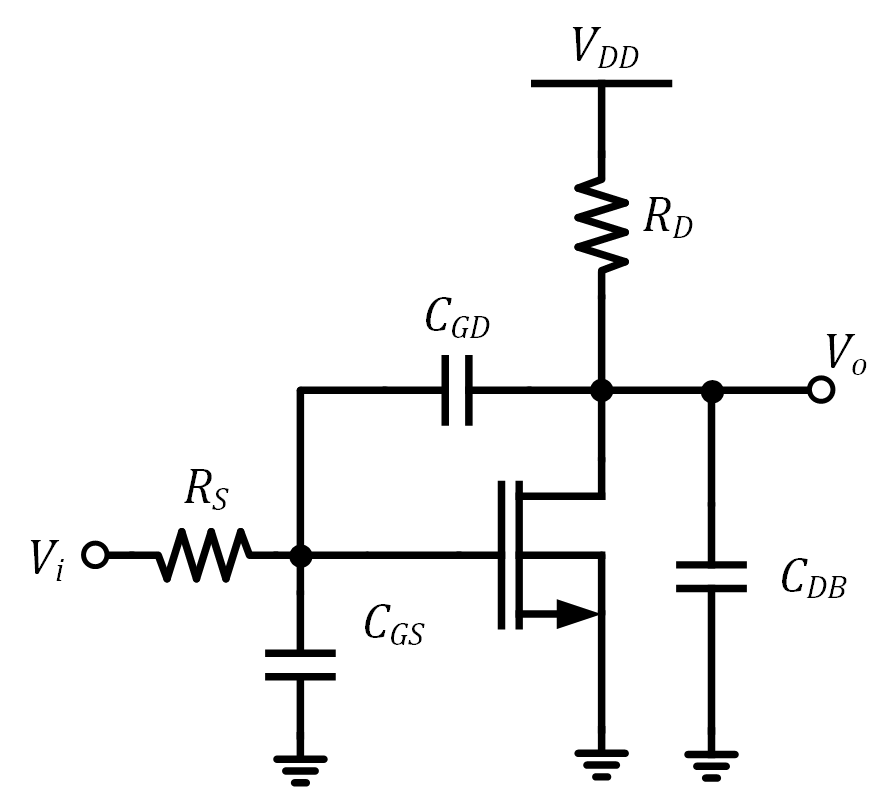
\includegraphics{common_source_AC.png}
\caption{common\_source\_AC.png}
\end{figure}

    \begin{equation}
\tau_1 = R_o C_{DB}  
\end{equation}

\begin{equation}
\tau_2 = R_S C_{GS}
\end{equation}

\begin{equation}
\tau_3 = (R_o + g_m R_S R_o + R_S) C_{GD}
\end{equation}

    \begin{equation}
\omega_{3dB} \approx \dfrac{1}{R_S(1+g_m R_o)C_{GD} + R_SC_{GS}+R_o(C_{DB}+C_{GD})}
\end{equation}

    \begin{itemize}
\tightlist
\item
  We arrive at an accurate expression for \(\omega_{p1}\) by an
  intuitive approach
\item
  The ZVTC method still has limitations (e.g.~when poles are close
  together)
\item
  We should combine the ZVTC method with SPICE/Cadence for design
\end{itemize}

    \hypertarget{dominant-pole-behavior}{%
\subsection{Dominant-pole behavior}\label{dominant-pole-behavior}}

    \begin{figure}
\centering
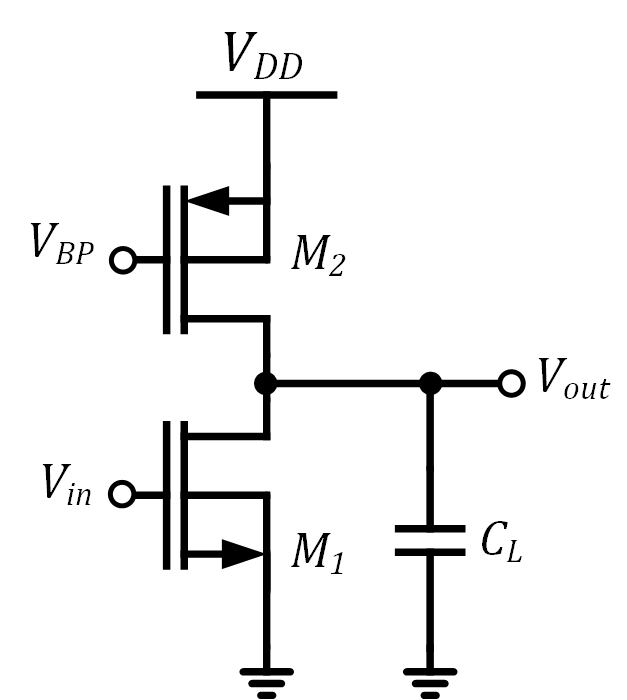
\includegraphics{active_common_source.png}
\caption{active\_common\_source.png}
\end{figure}

    \begin{itemize}
\tightlist
\item
  DC gain:
\end{itemize}

\begin{equation}
A_{v,DC} = -g_m R_o
\end{equation}

\begin{itemize}
\tightlist
\item
  Output pole:
\end{itemize}

\begin{equation}
\omega_{3dB} \approx \dfrac{1}{R_o C_L}
\end{equation}

    \begin{itemize}
\tightlist
\item
  For many applications we need to assume (or guarantee) that our
  amplifiers exhibit behavior similar to that of single-pole circuits
  (this is for stability reasons, which we'll discuss later)
\item
  We do this by ensuring one pole is ``dominant,'' i.e.~much lower in
  frequency than other poles
\item
  Here we are assuming that \(C_L\) is large enough for us to ignore
  other ``parasitic'' capacitances
\end{itemize}

    \hypertarget{gain-bandwidth-product}{%
\subsection{Gain-bandwidth product}\label{gain-bandwidth-product}}

    \begin{figure}
\centering
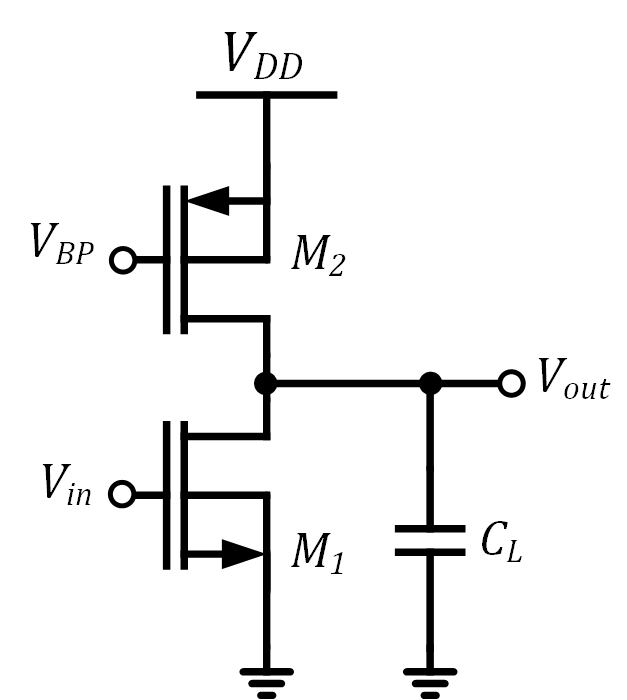
\includegraphics{active_common_source.png}
\caption{active\_common\_source.png}
\end{figure}

    \begin{itemize}
\tightlist
\item
  DC gain:
\end{itemize}

\begin{equation}
A_{v,DC} = -g_m R_o
\end{equation}

\begin{itemize}
\tightlist
\item
  Output pole:
\end{itemize}

\begin{equation}
\omega_{3dB} \approx \dfrac{1}{R_o C_L}
\end{equation}

    \begin{itemize}
\tightlist
\item
  If we assume dominant-pole behavior for the common-source amplifier,
  we can evaluate its gain-bandwidth product as
\end{itemize}

\begin{equation}
GBW \approx |A_{v,DC}|\cdot f_{3dB} = g_m R_o \cdot \dfrac{1}{2 \pi R_o C_L} = \dfrac{g_m}{2\pi C_L}
\end{equation}

\begin{itemize}
\tightlist
\item
  In many practical cases the gain-bandwidth product turns out to be a
  constant that is \emph{independent of output resistance}
\item
  This can be explained by the observation that as \(R_o\) increases,
  gain increases while bandwidth decreases, keeping their product
  constant
\end{itemize}

    \hypertarget{summary}{%
\subsection{Summary}\label{summary}}

    \begin{itemize}
\tightlist
\item
  The high-frequency behavior of MOS amplifiers is limited by intrinsic
  and extrinsic transistor capacitances
\item
  The frequency dependence of an amplifier's gain, input, and output
  impedances can be quantified in terms of poles and zeros contributed
  by those capacitances
\item
  The dominant pole of a common-source amplifier can be estimated via
  rigorous small-signal analysis, Miller's Theorem, or ZVTC analysis,
  though only the full small-signal transfer function can provide
  accurate assessments of non-dominant poles
\item
  When designing MOS analog circuits, we will use the dominant-pole
  approximation to provide an estimate of the gain-bandwidth product,
  and only include the effects of other ``non-dominant'' poles when
  analyzing stability
\end{itemize}


    % Add a bibliography block to the postdoc
    
    
    
\end{document}
